\documentclass[a4paper,12pt,twoside]{memoir}

% Castellano
\usepackage[spanish,es-tabla]{babel}
\selectlanguage{spanish}
\usepackage[utf8]{inputenc}
\usepackage[T1]{fontenc}
\usepackage{lmodern} % scalable font
\usepackage{microtype}
\usepackage{placeins}
\usepackage{float}
\usepackage{textcomp}
\usepackage{pdflscape}
\usepackage[justification=centering]{caption}
\usepackage{pgfgantt}

\RequirePackage{booktabs}
\RequirePackage[table]{xcolor}
\RequirePackage{xtab}
\RequirePackage{multirow}

% Links
\PassOptionsToPackage{hyphens}{url}\usepackage[colorlinks]{hyperref}
\hypersetup{
	allcolors = {red}
}

% Ecuaciones
\usepackage{amsmath}

% Rutas de fichero / paquete
\newcommand{\ruta}[1]{{\sffamily #1}}

% Párrafos
\nonzeroparskip

% Huérfanas y viudas
\widowpenalty100000
\clubpenalty100000

% Evitar solapes en el header
\nouppercaseheads


\let\tmp\oddsidemargin
\let\oddsidemargin\evensidemargin
\let\evensidemargin\tmp
\reversemarginpar



% Imagenes
\usepackage{graphicx}
\newcommand{\imagen}[2]{
	\begin{figure}[!h]
		\centering
		\includegraphics[width=0.9\textwidth]{#1}
		\caption{#2}\label{fig:#1}
	\end{figure}
	\FloatBarrier
}






\graphicspath{ {./img/} }

% Capítulos
\chapterstyle{bianchi}
\newcommand{\capitulo}[2]{
	\setcounter{chapter}{#1}
	\setcounter{section}{0}
	\setcounter{figure}{0}
	\setcounter{table}{0}
	\chapter*{#2}
	\addcontentsline{toc}{chapter}{#2}
	\markboth{#2}{#2}
}

% Apéndices
\renewcommand{\appendixname}{Apéndice}
\renewcommand*\cftappendixname{\appendixname}

\newcommand{\apendice}[1]{
	%\renewcommand{\thechapter}{A}
	\chapter{#1}
}

\renewcommand*\cftappendixname{\appendixname\ }

% Formato de portada
\makeatletter
\usepackage{xcolor}
\newcommand{\tutor}[1]{\def\@tutor{#1}}
\newcommand{\tutorb}[1]{\def\@tutorb{#1}}
\newcommand{\course}[1]{\def\@course{#1}}
\definecolor{cpardoBox}{HTML}{E6E6FF}
\def\maketitle{
  \null
  \thispagestyle{empty}
  % Cabecera ----------------
\begin{center}
  \noindent
\includegraphics[width=\textwidth]{cabeceraSalud}\vspace{1.5cm}%
\end{center}
  
  % Título proyecto y escudo salud ----------------
  \begin{center}
    \begin{minipage}[c][1.5cm][c]{.20\textwidth}
        
\includegraphics[width=\textwidth]{escudoSalud.pdf}
    \end{minipage}
  \end{center}
  
  \begin{center}
    \colorbox{cpardoBox}{%
        \begin{minipage}{.8\textwidth}
          \vspace{.5cm}\Large
          \begin{center}
          \textbf{TFG del Grado en Ingeniería de la Salud}\vspace{.6cm}\\
          \textbf{\LARGE\@title{}}
          \end{center}
          \vspace{.2cm}
        \end{minipage}
    }%
  \end{center}
  
    % Datos de alumno, curso y tutores ------------------
  \begin{center}%
  {%
    \noindent\LARGE
    Presentado por \@author{}\\ 
    en Universidad de Burgos\\
    \vspace{0.5cm}
    \noindent\Large
    \@date{}\\
    \vspace{0.5cm}
    Tutor: \@tutor{}\\ % comenta el que no corresponda
    %Tutores: \@tutor{} -- \@tutorb{}\\
  }%
  \end{center}%
  \null
  \cleardoublepage
  }
\makeatother



% Datos de portada
\title{Implementación del software de un pulsioxímetro externo integrado en la incubadora In$^3$ator \\Documentación Técnica}
\author{Elena Ruiz Moreno}
\tutor{Telmo Miguel Medina}
\tutorb{nombre tutor 2}
\date{\today}

\begin{document}

\maketitle



\cleardoublepage



%%%%%%%%%%%%%%%%%%%%%%%%%%%%%%%%%%%%%%%%%%%%%%%%%%%%%%%%%%%%%%%%%%%%%%%%%%%%%%%%%%%%%%%%



\frontmatter


\clearpage

% Indices
\tableofcontents

\clearpage

\listoffigures

\clearpage

\listoftables

\clearpage

\mainmatter

\appendix




\apendice{Plan de Proyecto Software}

\renewcommand{\arraystretch}{1.4}
\section{Introducción}

A continuación, se redacta la planificación llevada a cabo para desarrollar este proyecto. En primer lugar, a nivel temporal, se especifican las etapas de trabajo en forma de tareas. A nivel económico, se estiman los costes totales de cada parte implicada. Por último, a nivel legal, se indican las especificaciones requeridas para su desempeño.

\section{Planificación temporal}
Para la planificación temporal, se ha optado por utilizar un diagrama de Gantt, ya que el presente trabajo tiene un recorrido lineal y progresivo, no iterativo, y se ha realizado siguiendo un enfoque por fases de desarrollo técnico y de forma cronológica. 

Como paso previo a dicho diagrama, en la Tabla~\ref{tab:milestones} se recogen los principales hitos alcanzados durante el proyecto, junto con su correspondencia con las issues cerradas en el repositorio de GitHub\footnote{Link al repositorio de GitHub: \href{https://github.com/ElenaRuizMoreno/TFG-Elena-Ruiz/}{TFG - Elena Ruiz}}.

\vspace{0.3cm}
\begin{table}[H]
\centering
\renewcommand{\arraystretch}{1.1} % Reducido de 1.5 a 1.1
\begin{tabularx}{\textwidth}{|l|X|X|}
\hline
\textbf{Milestone} & \textbf{Descripción} & \textbf{Issues asociadas} \\
\hline
1 & Recopilación de información bibliográfica & \#1 \\
\hline
2 & Redacción de memoria con Latex & 
\#2, \#7, \#11, \#24, \#25, \#26, \#27, \#28, \#29 \\
\hline
3 & Configuración inicial del entorno de desarrollo y pruebas del pulsioxímetro & 
\#3, \#4, \#5, \#6 \\
\hline
4 & Análisis de datos crudos del sensor & 
\#8, \#9, \#10 \\
\hline
5 & Validación e implementación final de los algoritmos & \#12, \#14 \\
\hline
6 & Redacción de los anexos con Latex & 
\#13, \#15, \#18, \#19, \#20, \#21, \#22, \#23 \\
\hline
7 & Organización final del repositorio & 
\#16, \#17 \\
\hline
\end{tabularx}
\caption{Resumen de milestones del proyecto y issues asociadas. \textit{Elaboración propia.}}
\label{tab:milestones}
\end{table}


A continuación, se enumeran las tareas completadas hasta la fecha, con una breve descripción de cada una. 
\vspace{0.3cm}

\textbf{Recopilación de información bibliográfica}

Issue \textit{\#1 Búsqueda Bibliográfica.}

Periodo: 30/10/2024 - 10/04/2025.


\begin{itemize}
    \item Investigación sobre el funcionamiento de un pulsioxímetro y estado del arte de trabajos relacionados.
    \item Búsqueda de artículos y documentación sobre estimación de frecuencia cardíaca y saturación de oxígeno a partir de señales PPG.
\end{itemize}

\textbf{Configuración inicial del entorno de desarrollo y pruebas del pulsioxímetro}

Issue \textit{\#3 Seguimiento de comunicación y definición del alcance del pulsioxímetro.}

Periodo: 18/12/2024 - 20/02/2025.

\begin{itemize}
    \item Contacto con la organización para plantear el objetivo principal.
    \item Organización del envío y revisión del material proporcionado por la ONG \href{https://medicalopenworld.org/}{Medicina Abierta al Mundo}.
    \item Definición del alcance del pulsioxímetro en el sistema de incubadora y análisis del hardware disponible.
\end{itemize}

Issue \textit{\#4 Preparación del hardware: recepción y primeros ajustes.}

Periodo: 30/01/2025 - 05/03/2025.

Reuniones presenciales en el laboratorio para realizar pruebas de comunicación y validación del montaje de hardware.

\vspace{0.3cm}

Issue \textit{\#5 Instalación y configuración de los drivers del programador.}

Periodo: 11/02/2025 - 05/03/2025.

\begin{itemize}
    \item Instalación y configuración del entorno de desarrollo (Visual Studio Code + PlatformIO).
    \item Instalación de drivers necesarios para la conexión con la PCB.
\end{itemize}


Issue \textit{\#6 Captura y registro de datos crudos del sensor.}

Periodo: 02/03/2025 – 21/04/2025.

\begin{itemize}
    \item Desarrollo de varias versiones de una función concreta del firmware para registrar datos en un determinado periodo y frecuencia óptimos para su posterior análisis.
    \item Implementación de un script en Python para guardar datos del pulsioxímetro en formato CSV con inclusión de encabezados y una referencia al tiempo en ms.
    \item Sesiones de captura de datos con distintos resultados hasta conseguir los suficientes registros con la mejor calidad posible.
\end{itemize}

\textbf{Análisis de datos crudos del sensor.}

Issue \textit{\#8 Análisis de datos: Visualización de señales y siguientes pasos.}

Periodo: 10/03/2025 - 07/04/2025.

\begin{itemize}
    \item Lectura y visualización de los registros obtenidos.
    \item Clasificación de señales por calidad, y preparación para análisis cuantitativo.
\end{itemize}


Issue \textit{\#9 Cálculo de la frecuencia cardíaca a partir de los datos crudos del sensor.}

Periodo: 17/03/2025 - 05/04/2025.

\begin{itemize}
    \item Búsqueda de artículos y métodos relacionados con la estimación del valor de frecuencia cardíaca a partir de señales PPG procedentes de un pulsioxímetro.
    \item Implementación de diferentes métodos para detección de picos y cálculo de frecuencia cardíaca.
\end{itemize}


Issue \textit{\#10 Cálculo del valor de SpO$_2$ a partir de los datos crudos del sensor.}

Periodo: 07/04/2025 – 09/05/2025.

\begin{itemize}
    \item Documentación acerca de los principales métodos del cálculo de la saturación de oxígeno.
    \item Implementación de distintos algoritmos de cálculo (Ratio of Ratios, tabla LUT) en Python combinados con diferentes procesamientos.
\end{itemize}


\textbf{Validación e implementación final de los algoritmos}

Issue \textit{\#12 Análisis y optimización del tiempo de cómputo de los algoritmos de pulsioximetría.}

Periodo: 24/04/2025 - 13/05/2025.

Estudio del tiempo de cómputo de los algoritmos que mejores resultados ofrecían.

\vspace{0.3cm}

Issue \textit{\#14 Implementación en firmware de los algoritmos validados.}

Periodo: 09/05/2025 - 25/05/2025.

\begin{itemize}
    \item Adaptación del código Python a C++ para su inclusión en el firmware del ESP32.
    \item Pruebas con datos reales en entorno embebido.
\end{itemize}

\textbf{Redacción de la memoria con Latex}

\textit{\#2 Conceptos teóricos.}

Periodo: 18/01/2025 - 25/05/2025.

\begin{itemize}
    \item Desarrollo de los conceptos teóricos en la memoria teórica, que sirvió tanto para empezar a estructurar la memoria, como para dejar claros los fundamentos teóricos que definen el proyecto y así facilitar su comprensión.
\end{itemize}

Issue \textit{\#7 Comprensión y configuración de LaTeX para la memoria y anexos.}

Periodo: 05/03/2025 – 10/05/2025.

\begin{itemize}
    \item Descarga y adaptación de la plantilla oficial del TFG del grado de ingeniería de la salud.
    \item Comprensión básica de LaTeX, estructura de documentos, gestión de bibliografía y compilación.
\end{itemize}

Issue \textit{\#11 Redacción de la metodología.}

Periodo: 08/04/2025 – 02/06/2025.

\begin{itemize}
    \item Descripción de los datos utilizados a lo largo del proyecto, así como el proceso de adquisición de los mismos.
    \item Explicación de las herramientas hardware y software utilizadas.
    \item Documentación detallada del procedimiento experimental, filtros aplicados, y algoritmos utilizados.
\end{itemize}

Issue \textit{\#24 Resultados.}

Periodo: 03/06/2025 – 08/06/2025.

\begin{itemize}
    \item Resumen de los principales resultados obtenidos y breve explicación de los mismos a través de tablas de valores y gráficos demostrativos.
    \item Inclusión de capturas de pantalla del firmware que demuestran el funcionamiento del sistema, además de la referencia a un pequeño vídeo demostrativo de la solución desarollada en tiempo real.
\end{itemize}

Issue \textit{\#25 Conlcusiones.}

Periodo: 03/06/2025 – 08/06/2025

\begin{itemize}
    \item Presentación de las conclusiones obtenidas, relacionándolas con los objetivos del proyecto.
    \item Discusión de los resultados enfrentándolos a otros proyectos relacionados ya mencionados con anterioridad.
\end{itemize}

Issue \textit{\#26 Líneas de trabajo futuras.}

Periodo: 03/06/2025 – 08/06/2025.

Presentación de las principales líneas de trabajo que se consideran oportunas para continuar en un futuro con el sistema desarrollado y mejorarlo.

\vspace{0.3cm}

Issue \textit{\#27 Resumen.}

Periodo: 04/06/2025 – 08/06/2025.

\begin{itemize}
    \item Elaboración del resumen del trabajo sintentizando objetivos principales, metodología, resultados y conclusiones.
    \item Enumeración de las palabras clave relacionadas con el trabajo realizado.
\end{itemize}

Issue \textit{\#28 Introducción.}

Periodo: 05/06/2025 – 08/06/2025

Contextualización del problema a resolver por el sistema que se ha elaborado y breve explicación de como se ha abordado.

\vspace{0.3cm}

Issue \textit{\#29 Objetivos.}

Periodo estimado: 05/06/2025 – 08/06/2025

Enumeración del objetivo principal del proyecto planteado, objetivos personales y funcionales del sistema.

\newpage

\textbf{Organización final del repositorio}

Issue \textit{\#16 Clasificación de notebooks por validez de los métodos.}

Periodo: 13/05/2025 – 25/05/2025

\begin{itemize}
    \item Revisión de los notebooks desarrollados durante el análisis de frecuencia cardiaca y SpO$_2$.
    \item Evaluación de la validez de cada uno según señal de entrada, métricas, código y optimización.
    \item Eliminación o documentación de los notebooks no válidos, para evitar confusión en fases finales.
\end{itemize}

Issue \textit{\#17 Revisión y limpieza de notebooks definitivos.}

Periodo estimado: 13/05/2025 – 25/05/2025

\begin{itemize}
    \item Unificación del estilo y estructura de todos los notebooks definitivos del proyecto.
    \item Inclusión de comentarios explicativos para comprender lo que hace el código.
\end{itemize}

\textbf{Redacción de los anexos con Latex}

Issue \textit{\#13 Anexo A: Planificación del Proyecto.}

Periodo estimado: 24/05/2025 – 08/06/2025

\begin{itemize}
    \item Redacción del anexo que detalla la planificación temporal, económica y legal del proyecto.
    \item Relación entre las tareas descritas y las issues del repositorio de GitHub.
\end{itemize}

Issue \textit{\#15 Anexo D: Descripción y adquisición de los datos.}

Periodo estimado: 09/05/2025 – 08/06/2025

\begin{itemize}
    \item Documentación del procedimiento de captura y preprocesamiento de señales del pulsioxímetro.
    \item Explicación del formato de los ficheros CSV y descripción de la naturaleza de la señal registrada.
\end{itemize}

Issue \textit{\#18 Redacción del Anexo B: Documentación de Usuario.}

Periodo estimado: 25/05/2025 – 08/06/2025

\begin{itemize}
    \item Inclusión de requisitos software y hardware del sistema completo.
    \item Manual paso a paso para la instalación, ejecución y uso por parte de usuarios no técnicos.
\end{itemize}

Issue \textit{\#19 Redacción del Anexo C: Manual del Desarrollador.}

Periodo estimado: 25/05/2025 – 08/06/2025

\begin{itemize}
    \item Explicación de estructura de carpetas, herramientas utilizadas y dependencias.
    \item Documentación técnica para futuros desarrolladores del sistema.
    \item Instrucciones para compilar, modificar y validar el firmware y los scripts de análisis.
\end{itemize}

Issue \textit{\#20 Redacción del Anexo E: Especificación de Diseño.}

Periodo estimado: 25/05/2025 – 08/06/2025

\begin{itemize}
    \item Descripción del punto de partida del proyecto.
    \item Inclusión de diagramas de bloques, interfaz sensor-microcontrolador y resumen del algoritmo.
\end{itemize}

Issue \textit{\#21 Redacción del Anexo F: Especificación de Requisitos.}

Periodo estimado: 02/06/2025 – 08/06/2025

Adaptación del anexo a la naturaleza del proyecto y descripción del caso de uso principal.


Issue \textit{\#22 Redacción del Anexo G: Estudio experimental.}

Periodo estimado: 02/06/2025 – 08/06/2025

\begin{itemize}
    \item Descripción cronológica de todo lo realizado en forma de cuaderno de trabajo, incluyendo resultados negativos.
    \item Enumeración de los parámetros utilizados en los algoritmos.
\end{itemize}

Issue \textit{\#23 Redacción del Anexo H: Anexo de sostenibilización circular.}

Periodo estimado: 02/06/2025 – 08/06/2025

Identificación de los principales objetivos de desarrollo sostenible a los que se adhiere el proyecto realizado y explicar el por qué.

\begin{figure}[H]
    \centering
    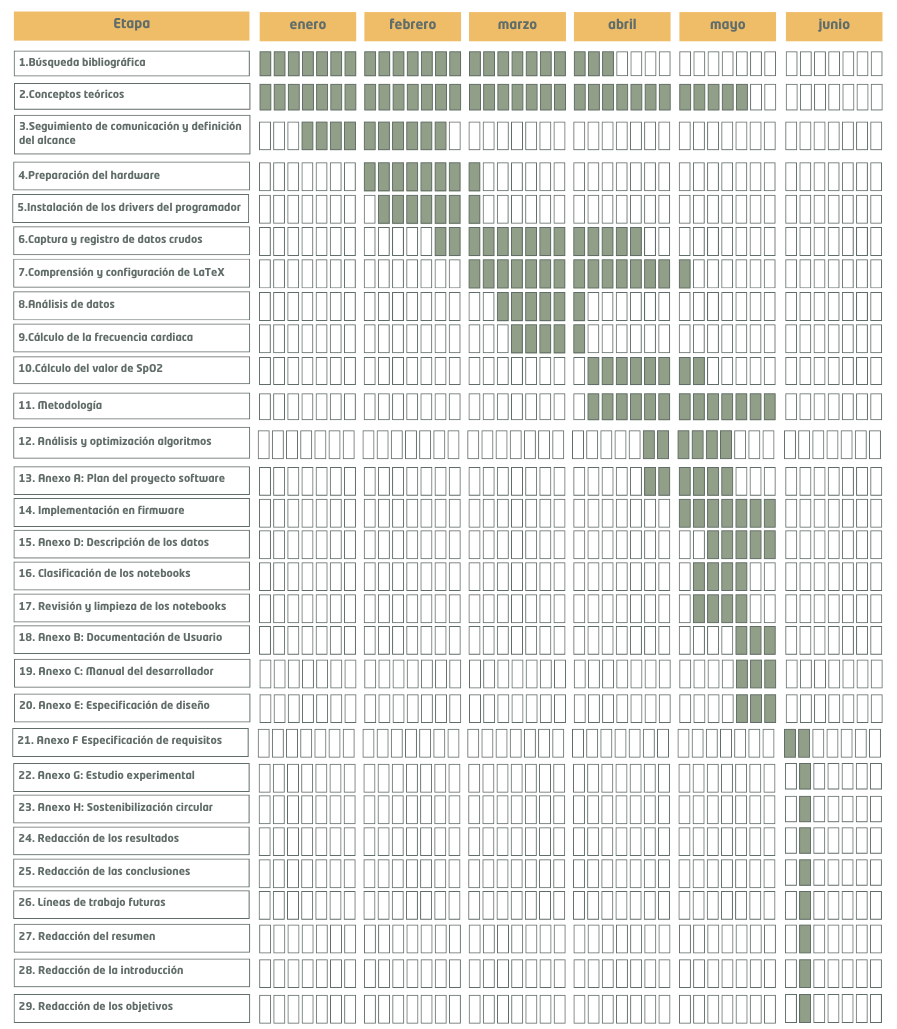
\includegraphics[width=0.9\linewidth]{img/DIAGRAMAGANTT.png}
    \caption{Representación de la planificación temporal seguida según las issues a partir de un diagrama de Gantt.\textit{ Elaboración propia.}}
    \label{fig:DIAGRAMAGANTT}
\end{figure}

\section{Planificación económica}
Se indican en este apartado los costes tanto personales como de
materiales, hardware y software necesarios.

\subsection{Costes personales}

Este proyecto se ha llevado a cabo completamente como parte de un Trabajo de Fin de Grado sin recibir compensación económica directa por ello. Sin embargo, para poder reflejar el valor técnico y hacer una comparación realista con su desarrollo en un entorno profesional, se ha calculado el coste equivalente al tiempo de trabajo que se ha invertido.

Para estimar este coste, se ha tomado como referencia el salario bruto medio de entrada en el mercado laboral para un perfil de ingeniería recién graduado en España, situado en torno a los 25.000 € brutos anuales a jornada completa \cite{ufv:salario}. Esto equivale a un salario mensual bruto de aproximadamente 1.763 € (en 14 pagas), con un salario neto estimado en torno a 1.500 € tras aplicar las deducciones correspondientes.

Debido a que para el desarrollo de este proyecto se ha trabajado una media de 4 horas diarias, distribuidas en 5 días a la semana, se considera equivalente a una jornada parcial (media jornada) típica de un ingeniero junior.

Partiendo de un salario bruto anual de 25.000 € para una jornada completa, el salario bruto anual estimado para una jornada parcial equivalente (media jornada) se reduce a la mitad:

\[
\frac{25.000 \text{€}}{2} = \textbf{12.500 €}
\]

Considerando una jornada parcial de 4 horas al día durante 5 días a la semana, teniendo 42 semanas laborales al año:

\[
4\,\text{h/día} \times 5\,\text{días/sem} \times 42\,\text{sem} = \textbf{840\,h/año}
\]

De ahí se obtiene el coste por hora bruto:

\[
\frac{12.500 \text{€}}{840\,h} = \textbf{14{,}88 €/h}
\]

Aplicando una retención del 16\% (factor 0,84) para IRPF y cotizaciones sociales, se obtiene el coste por hora neto:

\[
14{,}88 \text{€} \times 0{,}84 = \textbf{12{,}50 €/h}
\]


\begin{table}[H]
\centering
\begin{tabular}{|l|c|}
\hline
\textbf{Concepto} & \textbf{Valor} \\
\hline
Salario bruto anual estimado (media jornada) & 12.500 € \\
Horas anuales estimadas (media jornada) & 840 h \\
Coste por hora (bruto) & 14{,}88 €/h \\
Coste por hora (neto) & 12{,}5 €/h\\
\hline
\end{tabular}
\caption{Estimación del coste por hora a media jornada de un ingeniero recién graduado.}
\label{tab:coste_hora}
\end{table}

A partir del seguimiento real del trabajo realizado durante el proyecto, se estima una dedicación total de aproximadamente 480 horas efectivas distribuidas a lo largo de seis meses. Esta estimación contempla tareas técnicas, adquisición de señales, validación de algoritmos y redacción de la documentación. No se han incluido en este cómputo las actividades relacionadas con el desarrollo previo de la placa base y el firmware completo de la incubadora, ya que se ha partido de este material ya desarrollado por la organización.

Aplicando el coste por hora neto estimado, el coste personal total equivalente asciende a:

\[
480 \, \text{h} \times 12,5\, \frac{\text{€}}{\text{h}} = \textbf{6.000\,€}
\]


\subsection{Costes de herramientas utilizadas}

Durante el proyecto se ha utilizado, por una parte, equipamiento propio y por otra, material prestado de la ONG Medicina Abierta al Mundo.  A continuación, se detallan los costes amortizados de dichos recursos, suponiendo una vida útil de 4 años y una utilización de 6 meses.

Dado que se trata de un desarrollo centrado en software, la herramienta principal empleada ha sido un ordenador portátil:

\begin{table}[H]
\centering
\begin{tabular}{|l|c|c|}
\hline
\textbf{Concepto} & \textbf{Precio total} & \textbf{Amortización 6 meses} \\
\hline
Ordenador portátil HP Core i5 & 600 €\footnotemark[1] & 75 € \\
Licencia Office 365 anual & 99 €\footnotemark[2] & 49,5 € \\
\hline
\textbf{Total} & 699 € & \textbf{124,5 €} \\
\hline
\end{tabular}
\caption{Costes de las herramientas personales amortizados a 6 meses.}
\label{tab:costes-amortizados}
\end{table}


\footnotetext[1]{Precio de referencia de la gama HP Core i5 consultado en la página oficial de HP \cite{hp2024}.}
\footnotetext[2]{En nuestro caso, la licencia Office 365 está cubierta por la Universidad de Burgos, pero en el peor de los casos, el precio de la suscripción a Office 365 personal anual, está disponible en la web de Microsoft \cite{microsoft2024}.}




\subsubsection{Costes de materiales para el prototipo}

El sistema fue validado con un prototipo basado en una PCB que simulaba la incubadora y complementado con electrónica de apoyo  facilitada por la ONG:

\begin{table}[H]
\centering
\begin{tabular}{|l|c|c|}
\hline
\textbf{Elemento} & \textbf{Precio (2025)} & \textbf{Proveedor} \\
\hline
PCBA (Placa electrónica) & 60,00 € & JLCPCB\footnotemark[3] \\
Display táctil 7”         & 40,00 € & Elecrow\footnotemark[4] \\
Fuente alimentación 12V (20A mín.) & 9,00 € & Alibaba\footnotemark[5] \\
Cable microUSB  & 4,78 € & StarTech\footnotemark[6] \\
Sensor UA401-D (pulsioxímetro) & 13,69 € & Alibaba\footnotemark[5] \\
Cable IEC C13 europeo 3 metros & 2,00€ & Alibaba\footnotemark[5] \\
Enchufe CA IEC320 (C14 AC-04) & 2,20€ & AliExpress\footnotemark[7] \\
Placa de desarrollo ESP-Prog & 16,76€ & AliExpress \footnotemark[7] \\
Pulsioxímetro comercial 1 & 12,46 € & Berrcom\footnotemark[8]\\
Pulsioxímetro comercial 2 & 28,99 € & Dr. Senst\footnotemark[9]\\
\hline
\textbf{Total} & \textbf{189,88 €} & \\
\hline
\end{tabular}
\caption{Costes actualizados de los materiales del sistema de pulsioximetría (precios 2025).}
\label{tab:costes_pulsioximetro}
\end{table}

\footnotetext[3]{Consultar aquí \href{https://jlcpcb.com}{JLCPCB}}
\footnotetext[4]{Consultar aquí \href{https://www.elecrow.com}{Elecrow}}
\footnotetext[5]{Consultar aquí \href{https://www.alibaba.com}{Alibaba}}
\footnotetext[6]{Consultar aquí \href{https://www.startech.com/}{StarTech}}
\footnotetext[7]{Consultar aquí \href{https://www.aliexpress.com/}{AliExpress}}
\footnotetext[8]{Consultar aquí \href{https://www.berrcomonline.com}{Berrcom}}
\footnotetext[9]{Consultar aquí \href{https://www.dr-senst.com/}{DrSenst}}



\noindent Los costes de cada componente han sido solicitados al responsable del proyecto, que nos lo ha cedido. 

\subsection{Resumen de costes estimados}

\begin{table}[H]
\centering
\begin{tabular}{|l|c|}
\hline
\textbf{Categoría} & \textbf{Coste } \\
\hline
Coste personal estimado            & 6.000€ \\
Herramientas y software (amortizado) & 124{,}5€ \\
Materiales y hardware del prototipo & 189,88€ \\
\hline
\textbf{Total estimado}             & \textbf{6.314,38€} \\
\hline
\end{tabular}
\caption{Resumen del coste económico del proyecto.}
\label{tab:coste_total}
\end{table}

\noindent Este coste no contempla producción en serie ni certificación sanitaria. Si el sistema se escalase para su implementación real en incubadoras clínicas, sería necesario incorporar gastos de validación normativa, fabricación, I+D adicional y soporte técnico.


\section{Viabilidad legal}

En este apartado se analizan las normativas relacionadas con el uso de datos, la distribución del software, y las posibles exigencias regulatorias si el sistema evolucionara hacia un dispositivo médico integrado en un entorno clínico real. 

\vspace{0.3cm}
\subsection{Uso de datos biomédicos}

Durante el desarrollo del sistema se han utilizado datos de señales ópticas  generadas a partir de pruebas con parámetros fisiológicos propios. En ningún momento se han utilizado datos de pacientes ni información sensible o identificativa. Todos los registros utilizados (valores de pulsioximetría) se almacenaron de forma local y sin vinculación a personas concretas, cumpliendo así con el Reglamento General de Protección de Datos (RGPD, UE 2016/679) y la LOPDGDD española (Ley Orgánica 3/2018).

\begin{itemize}
    \item El \textbf{Reglamento General de Protección de Datos} (\textbf{RGPD}, Reglamento (UE) 2016/679)\cite{rgpd2016}, establece las condiciones legales para el tratamiento de datos personales dentro de la Unión Europea. Aunque este trabajo no implica datos identificativos, se ha respetado el principio de minimización y anonimización exigido por el reglamento.
    
    \item La \textbf{Ley Orgánica 3/2018}, de Protección de Datos Personales y garantía de los derechos digitales (\textbf{LOPDGDD})\cite{lopd2018}, adapta el RGPD al contexto jurídico español e introduce medidas específicas para entornos educativos y de investigación. En este sentido, se cumple con las condiciones que permiten el uso de datos biomédicos anonimizados para fines académicos sin requerir consentimiento explícito, garantizando en todo momento la protección de la privacidad.
\end{itemize}

\vspace{0.3cm}
\subsection{Licencias del software empleado}

Todas las herramientas que se han utilizado durante el desarrollo del proyecto han sido de software libre y de código abierto. Las plataformas utilizadas permiten su uso gratuito como parte de un contexto académico y de investigación, sin necesidad de licencias comerciales.

El código fuente generado se encuentra disponible públicamente en GitHub \footnote{\href{https://github.com/ElenaRuizMoreno/TFG-Elena-Ruiz}{TFG-ElenaRuiz}} bajo una licencia tipo MIT, lo que permite su uso, distribución y modificación con fines no comerciales, siempre y cuando se haga referencia al autor correspondiente.

Además, cabe destacar que este trabajo parte de una base de código y hardware previamente desarrollados por la ONG \href{https://medicalopenworld.org/}{Medicina Abierta al Mundo}, con la que se ha mantenido contacto directo durante el desarrollo. En concreto, el firmware de la incubadora (incluido el archivo \texttt{SPO2.cpp}, que es el que implementa el funcionamiento para el cálculo de la frecuencia cardíaca y la saturación de oxígeno) se encuentra publicado en el repositorio oficial de la ONG en GitHub \footnote{\href{https://github.com/medicalopenworld/in3ator}{medicalopenworld}}.

Dado que dicho repositorio es público y de acceso libre, su uso como base para la implementación del código y para la extracción de los datos utilizados no infringe ninguna restricción legal, siempre que se mencione la autoría original, lo cual ha sido respetado.

\vspace{0.3cm}

\subsection{Regulación aplicable en caso de evolución a dispositivo médico}

Aunque el sistema desarrollado en este proyecto no está destinado a un uso clínico real en su estado actual, se plantea su integración futura en una incubadora neonatal distribuida por la ONG Medicina Abierta al Mundo. En este contexto, sería obligatorio que el sistema cumpla con algunas de las leyes específicamente planteadas para dispositivos sanitarios.

\begin{itemize}
    \item El \textbf{Reglamento (UE) 2017/745} sobre productos sanitarios (MDR)  \cite{mdr2017} establece los requisitos legales para la comercialización y uso de dispositivos médicos en Europa. En el caso de que el pulsioxímetro, fuera viable y realmente monitorizara de forma eficaz los parámetros necesarios para el control de un neonato, pasaría a ser considerado un dispositivo médico, y sería necesario que fuera sometido a procesos de certificación, validación clínica y control de calidad, incluyendo la evaluación de riesgos, la documentación técnica, y la obtención del marcado CE\footnote{El marcado CE (Conformité Européenne) es un sello de conformidad obligatorio que indica que el producto ha sido evaluado y cumple con los requisitos esenciales de seguridad, salud, medio ambiente y rendimiento establecidos en las directivas europeas. }. 

    \item La \textbf{norma ISO 13485}\cite{iso13485} especifica los requisitos que debe cumplir un sistema de gestión de calidad para fabricantes y desarrolladores de dispositivos médicos. Si la ONG finalmente escala este proyecto, debería implementar un sistema de acuerdo a esta norma para garantizar el control de la seguridad y fiabilidad de su uso.

    \item Finalmente, la \textbf{norma IEC 80601-2-61:2017}\cite{iec80601}, que resulta especialmente relevante, ya que regula la seguridad y rendimiento específicos para pulsioxímetros. Esta norma establece, por ejemplo, los márgenes de precisión tolerables, los métodos de validación mediante estudios en voluntarios humanos y las pruebas eléctricas y electromagnéticas requeridas para que no cause interferencias con perturbaciones externas. Cualquier futura implementación debería cumplir todos estos requisitos para poder ser integrado en una incubadora que es utilizada en un hospital.

\end{itemize}



\apendice{Documentación de usuario}

\section{Instalación / Puesta en marcha}

Este sistema ha sido diseñado para monitorizar, de forma sencilla y en tiempo real, dos parámetros vitales del neonato: la saturación de oxígeno y la frecuencia cardíaca. Por lo tanto, el usuario, idealmente, debería ser un médico o un enfermero que sea responsable del control de estos pacientes en ambientes como hospitales o UCIs neonatales. Aunque no se ha conseguido un objetivo final lo suficientemente fiable como para ser utilizado en un entorno real, a continuación se explica, de forma clara y práctica, cómo se colocaría el sensor y cómo interpretar lo que aparece en la pantalla como si el sistema ya estuviese integrado en la incubadora.

\subsection{Paso 1: Preparación y encendido de la incubadora}

\begin{itemize}
    \item Seguir primero las instrucciones del manual de la incubadora \textit{In$^3$ator} \footnote{El manual mencionado disponible en \href{https://ayudacontenedores.org/storage/2021/11/in3ator_user_manual-v1.0-Spanish.pdf}{Ayuda Contenedores.}}(capítulo “2.5 Panel de operación”):
    \begin{itemize}
        \item Conectar la fuente de alimentación de 12V a la cuna climática.
        \item Colocar una botella de agua nueva en el humidificador (se recomienda usar agua destilada o embotellada, nunca del grifo).
        \item Conectar el cable del humidificador a la toma correspondiente.
        \item Encender la cuna usando el interruptor general.
        \item En el menú principal o avanzado, seleccionar el modo operativo deseado:
        \begin{itemize}
            \item Configurar las semanas de gestación o ajustar manualmente la temperatura y humedad (según el caso).
            \item Activar los LEDs si se desea aplicar fototerapia.
            \item Pulsar el botón “Inicio” (Aparece una vez se configuran las opciones que señala).
            \begin{figure}[H]
            \centering
            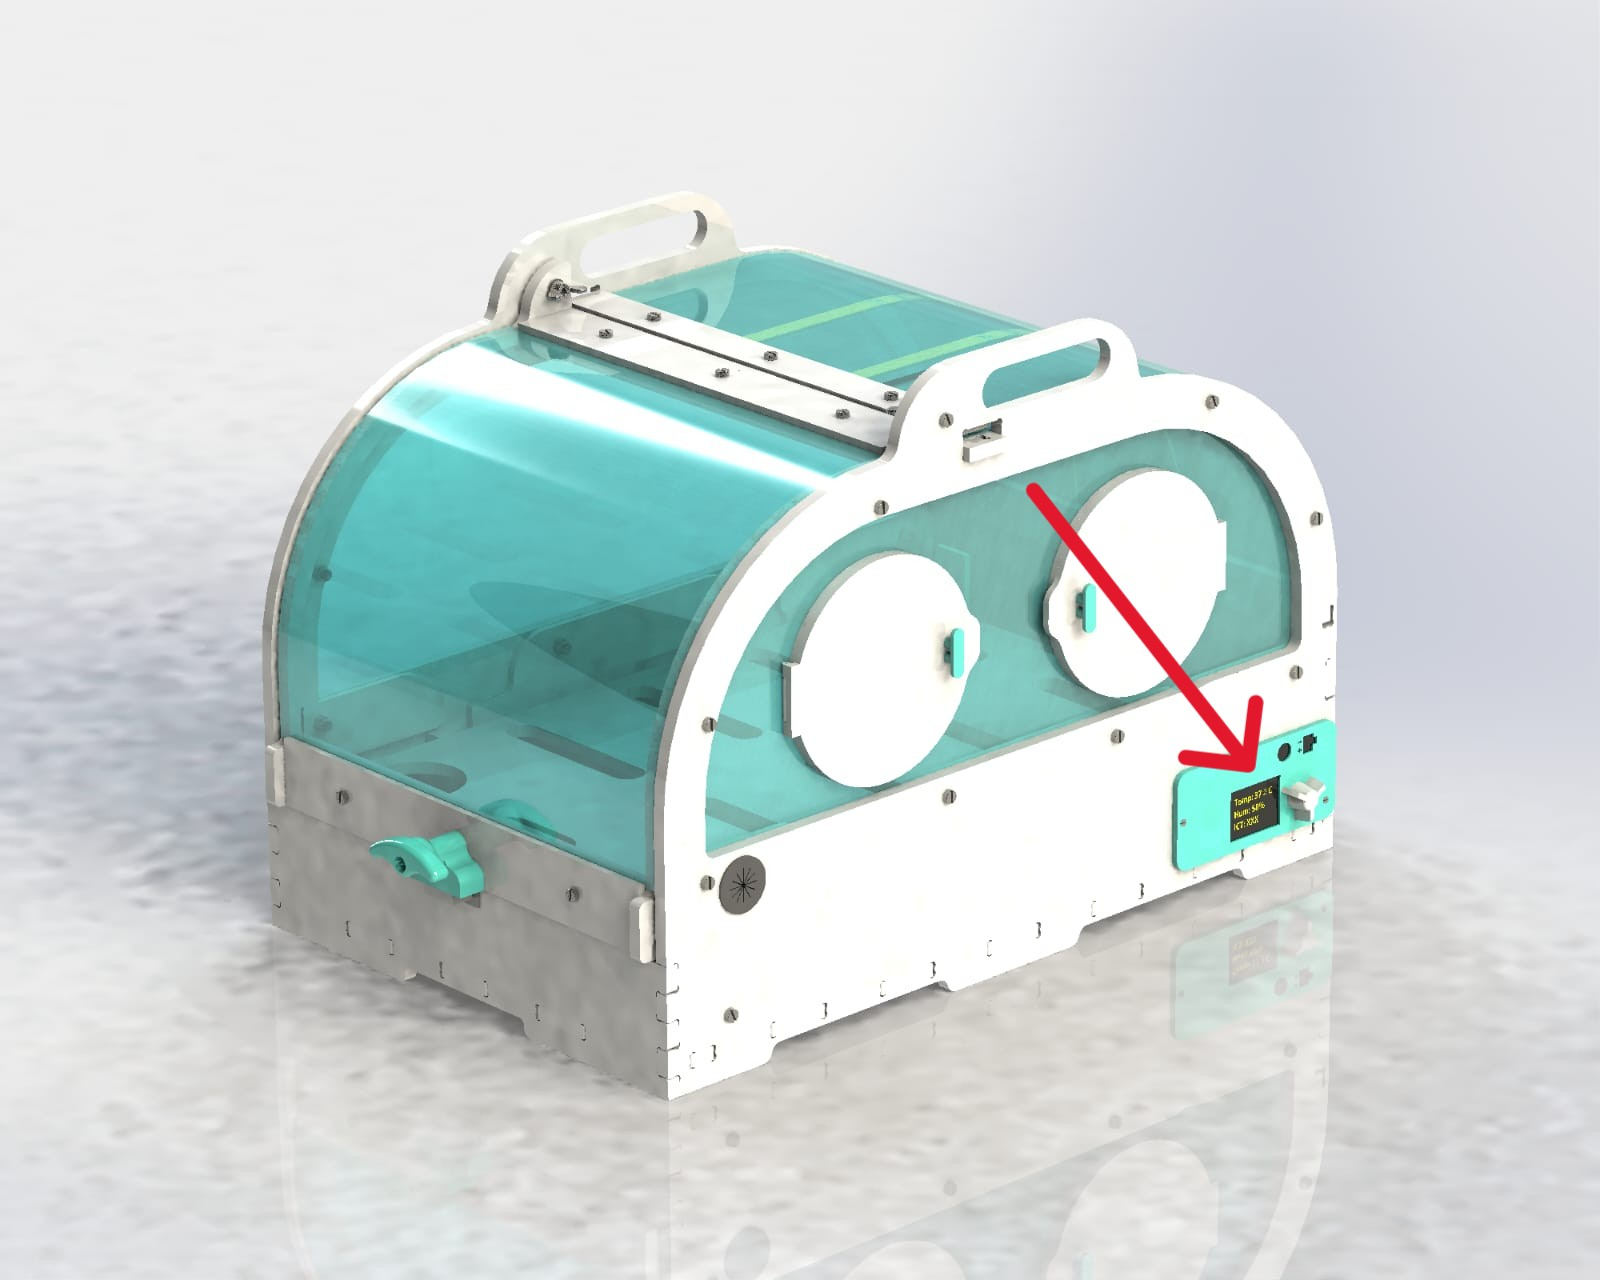
\includegraphics[scale=0.15]{img/incubadora.jpeg}
            \caption{Ubicación de la pantalla en la incubadora. Fuente adaptada: \href{https://medicalopenworld.org/la-incubadora/}{MedicalOpenWorld}}
            \label{fig:pantalla_incubadora}
            \end{figure}
    
            \begin{figure}[H]
            \centering
            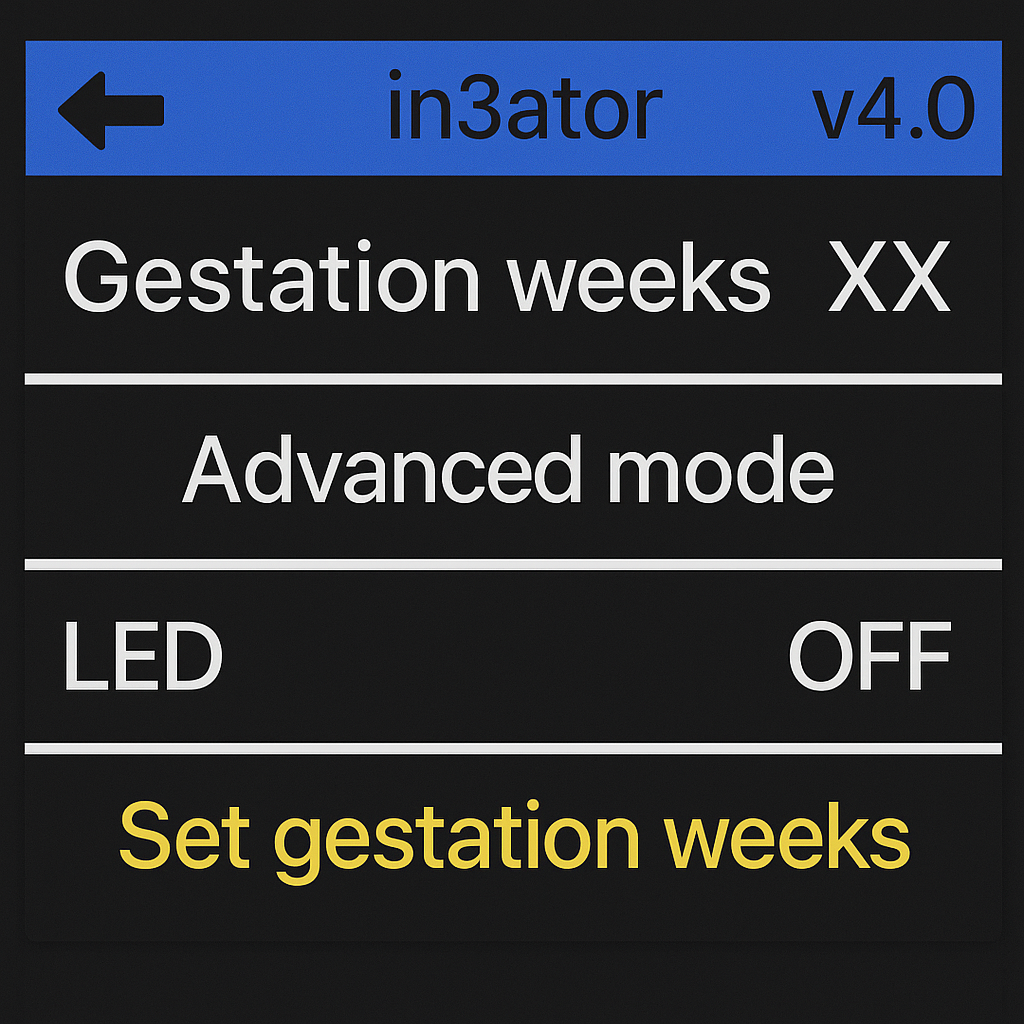
\includegraphics[scale = 0.13]{img/menu_display.png}
            \caption{Display inicial de la incubadora. Fuente adaptada: \href{https://ayudacontenedores.org/storage/2021/11/in3ator_user_manual-v1.0-Spanish.pdf}{Ayuda Contenedores.} }
            \label{fig:display}
            \end{figure}
        \end{itemize}
    \item Si es posible, dejar la cuna precalentando durante al menos 30 minutos antes de introducir al bebé.
    \end{itemize}
\end{itemize}

\subsection{Paso 2: Colocación del sensor óptico}

\begin{itemize}
    \item Antes de manipular al neonato, asegurar que la incubadora mantiene las condiciones térmicas y de humedad recomendadas.
    \item Comprobando que el sensor U401-D se encuentra bien enchufado a su puerto correspondiente, colocarlo:
    \begin{itemize}
        \item En una zona acral\footnote{La definición de “acral” es “superior” o “más alto”, y este término se refiere a una parte del cuerpo que está más alejada del centro, es decir, en los extremos de los brazos o las piernas} del paciente (pie, palma de la mano, orejas o nariz), tal como se aconseja para minimizar interferencias.
        \item Usar la cinta regulable que incluye el sensor para fijarlo sin apretar demasiado.
        \begin{figure}[H]
            \centering
            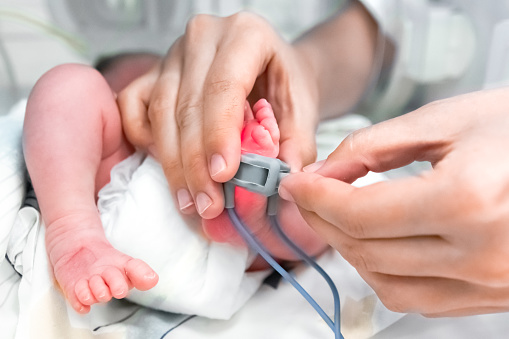
\includegraphics[width=0.4\linewidth]{img/medico.jpg}
            \caption{Ejemplo de la posición prevista para el sensor óptico. Fuente: \cite{semianovich2020oximetro}. }
            \label{fig:medico}
        \end{figure}
    \end{itemize}
\end{itemize}

\subsection{Paso 3: Visualización de los parámetros en pantalla}

\begin{itemize}
    \item En la pantalla de la incubadora, junto con los campos habituales de temperatura y humedad, se mostrará también la lectura en tiempo real de:
        \begin{itemize}
            \item Saturación de oxígeno (SpO$_2$)
            \item Frecuencia cardíaca 
            \begin{figure}[H]
            \centering
            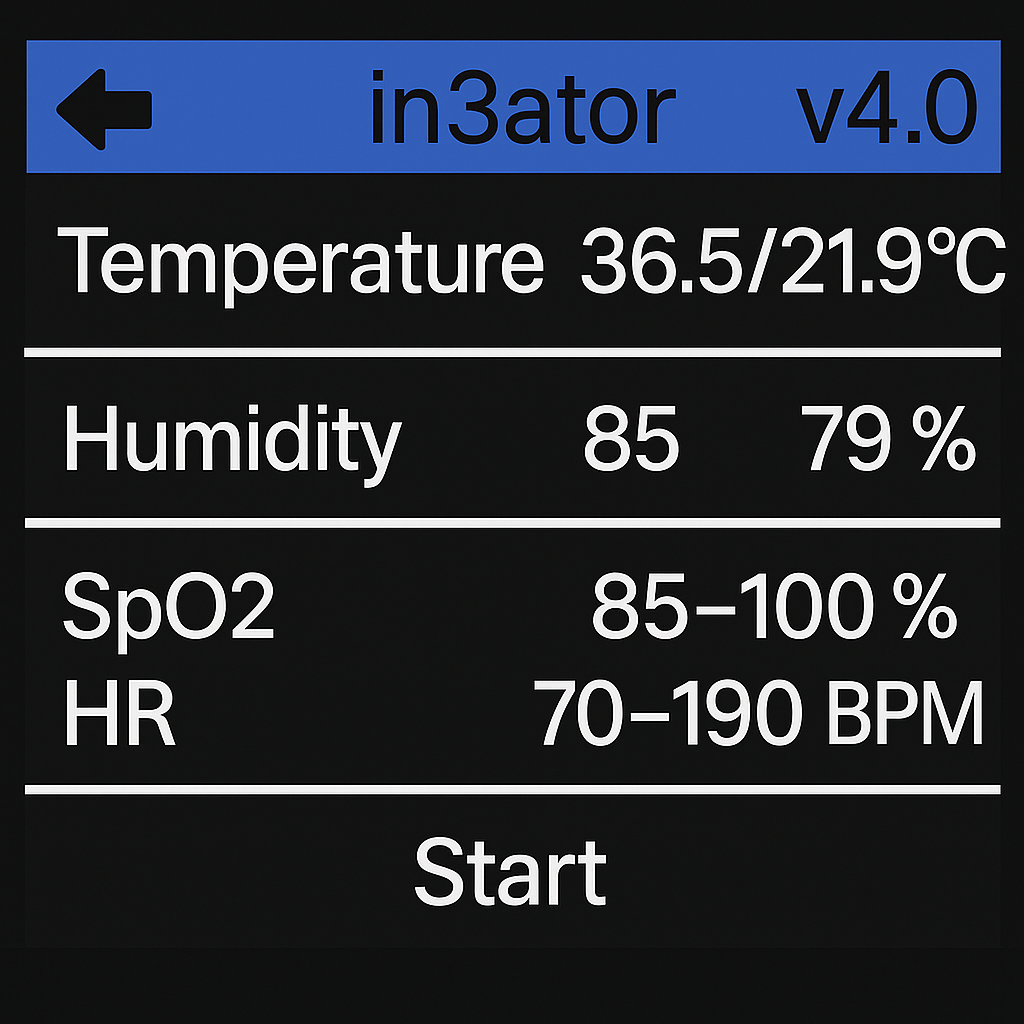
\includegraphics[scale = 0.13]{img/display.png}
            \caption{Display que muestra los parámetros que controla la incubadora. Fuente adaptada: \textit{Elaboración propia.}}
            \label{fig:display}
            \end{figure}
        \end{itemize}
    \item Estos valores pueden tardar algunos segundos en estabilizarse después de conectar el sensor.
    \item Valores normales esperados:
        \begin{itemize}
            \item \textbf{SpO$_2$:} 85–100\%
            \item \textbf{Frecuencia cardíaca:} 70-190 bpm
        \end{itemize}
    \item Si los valores se muestran inestables, parpadean, o aparecen líneas discontinuas o símbolos de error:
        \begin{itemize}
            \item Verificar que el sensor esté bien colocado.
            \item Asegurar de que el neonato esté tranquilo y que no haya movimiento excesivo.
            \item Evitar fuentes de luz intensa apuntando directamente al sensor.
        \end{itemize}
\end{itemize}

\subsection{Paso 4: Apagado del sistema o cambio de configuración}

\begin{itemize}
    \item Para detener el funcionamiento del sistema, presionar el codificador rotatorio\footnote{El codificador rotatorio es el botón giratorio situado a la derecha de la pantalla. Permite navegar por el menú girándolo, y confirmar opciones pulsándolo } durante 2 segundos (esto lleva al menú principal).
    \item Si es necesario modificar algún parámetro, acceder al modo avanzado manteniendo pulsado el codificador durante más de 5 segundos.
    \item Para apagar completamente la incubadora, desenchufar la fuente de alimentación.
\end{itemize}

\section{Manual de interpretación de los resultados obtenidos}

Los valores que muestra el sistema están diseñados para ofrecer una lectura rápida y clara del estado del neonato. En esta versión, los parámetros monitorizados son:

\begin{itemize}
    \item \textbf{SpO$_2$ (saturación de oxígeno):} se muestra como un porcentaje (\%).
    \item \textbf{HR (frecuencia cardíaca):} se muestra en pulsaciones por minuto (BPM).
\end{itemize}

\subsection{Valores de referencia esperados}

Los rangos normales pueden variar ligeramente según el estado clínico del paciente, pero en general se consideran adecuados los siguientes valores:

\begin{itemize}
    \item \textbf{SpO$_2$:} entre 85\% y 100\%. \\
    Valores por debajo de 90\% indican hipoxemia y requieren evaluación inmediata.
    
    \item \textbf{HR:} entre 120 y 160 BPM en neonatos sanos. \\
    Valores persistentemente por debajo de 100 BPM o por encima de 180 BPM pueden indicar bradicardia o taquicardia, respectivamente.
\end{itemize}


\section{Manuales y/o Demostraciones prácticas}

Aunque este anexo está enfocado a cómo podría usarse el sistema en un entorno clínico real en el futuro, también se ha incluido un vídeo complementario que muestra parte del trabajo realizado durante el desarrollo.

En el vídeo se puede ver una demostración práctica donde se compara el funcionamiento del sensor óptico conectado a la placa con un pulsioxímetro comercial. Para ello, me coloco el pulsioxímetro comercial en una mano y el sensor óptico que ejecuta el software desarrollado en la otra, y se registran los datos en tiempo real mientras se visualizan en la consola de Visual Studio Code. Esto permite comprobar que las lecturas obtenidas con ambos sistemas son similares en condiciones normales.

El vídeo está disponible en el repositorio del proyecto, en la siguiente ruta:

\begin{center}
\texttt{TFG-Elena-Ruiz/Demostraci\'on/TFG\_ElenaRuiz.mp4}
\end{center}

Este contenido no forma parte del manual clínico, pero puede ser útil para entender mejor cómo funciona el sistema y cómo se ha comprobado su comportamiento durante el desarrollo.



    
     
\apendice{Manual del desarrollador} 

\section{Estructura de directorios}

El proyecto se ha organizado en una estructura de carpetas diferenciadas. A continuación, se describe el contenido y propósito de cada directorio:

\begin{itemize}
    \item \textbf{Artículos}: contiene una recopilación de artículos científicos y documentación técnica utilizada para la elaboración del estado del arte y la justificación de decisiones técnicas a lo largo del TFG. Dentro de ella, además de diferentes técnicas y métodos, hay un subdirectorio llamado \texttt{TFGs Pulsioxímetro}, en el que se pueden encontrar diferentes trabajos o proyectos que han desarrollado soluciones similares y que han servido de ayuda para entender cómo se han abordado problemas parecidos y qué soluciones se han propuesto en otros contextos.

   \item \textbf{Código}: incluye todos los scripts, algoritmos y archivos fuente del proyecto. Está dividido en subcarpetas:
\begin{itemize}

    \item \textbf{adquisición:} Contiene los scripts de Python que hay que ejecutar en el promt de Anaconda para poder registrar los datos y guardarlos en local en formato .csv en la ruta que se indique.
    
    \item \textbf{comparación}: contiene scripts para comparar los diferentes filtros descritos en el apartado de conceptos teóricos. Además, realiza una representación gráfica para observar el efecto de cada filtro sobre una señal PPG de ejemplo.
    
    \item \textbf{diagramas de bloques}: incluye esquemas visuales que representan el funcionamiento de los algoritmos y la arquitectura general del sistema.

    \item \textbf{firmware}: contiene el código embebido \textbf{original} que se ejecuta en la PCB de la incubadora. 

    \item \textbf{funciones modificadas:} en este directorio se encuentran los archivos \texttt{get\_AFE44XX\_Data\_modificada.cpp}, para la recogida de datos y \texttt{SPO2\_modificado.cpp}, que implementa el algoritmo de estimación de constantes fisiológicas. 
    
    \item \textbf{procesamiento}: contiene notebooks y scripts de Python para el tratamiento, filtrado y análisis de las señales registradas. También se calculan aquí los parámetros fisiológicos. Está organizado en dos carpetas principales, una para cada parámetro estimado, y dentro de cada una de ellas hay subcarpetas con pruebas, incluyendo procedimientos descartados.

    \item \textbf{resultados}: recoge las gráficas y tablas generados a partir del análisis de los algoritmos implementados en Python.
\end{itemize}


    \item \textbf{Datos}: estructura donde se almacenan los datos recogidos durante las sesiones de prueba. Se organiza en:
    \begin{itemize}
        \item \textbf{Datos crudos}: señales originales sin procesar. Se dividen en los directorios \texttt{save\_log} y \texttt{save\_log2}, según la versión de la función de adquisición que se haya utilizado.
        \item \textbf{Datos\_limpios}: señales tras la limpieza inicial, con un recorte \textbf{personalizado} para cada registro, según lo que sobrara de cada señal.
        \item \textbf{Procesados}: datos limpios, pero habiendo recortado para todos los registros, los primeros y últimos 5 segundos.
    \end{itemize}

    \item \textbf{Demostración}: vídeo corto de una simulación funcional de la solución desarrollada (formato \texttt{.mp4}).

    \item \textbf{Documentación de referencia}: manuales técnicos de los componentes utilizados (AFE4490, sensor UA401-D, normas ISO aplicables, documentación del proyecto \textit{In$^3$ator}, etc.). La mayoría cedidos por la ONG Medicina Abierta al Mundo.

    \item \textbf{Documentación Overleaf}: este es el proyecto principal en Overleaf donde se redacta tanto la memoria del TFG como los anexos. Está organizado en las siguientes carpetas y archivos:

    \begin{itemize}
        \item \texttt{tex/}: contiene los archivos `.tex` que forman los distintos capítulos de la memoria (introducción, metodología, resultados, etc.). 
        \item \texttt{img/}: carpeta con las imágenes, figuras y diagramas utilizados a lo largo del documento.
        \item \texttt{memoria.tex}: archivo principal que compila toda la memoria del TFG importando los capítulos desde la carpeta \texttt{tex}.
        \item \texttt{anexos.tex}: archivo donde se redactan todos los anexos del trabajo, también de forma modular.
        \item \texttt{bibliografia.bib}: fichero BibTeX con las referencias bibliográficas utilizadas en la memoria principal.
        \item \texttt{bibliografiaAnexos.bib}: archivo separado con las referencias citadas únicamente en los anexos, para mantener la bibliografía organizada y evitar duplicidades.
    \end{itemize}


    \item \textbf{README.md}: archivo de texto que resume el propósito del trabajo y explica brevemente cómo utilizar el proyecto.

    
    
\end{itemize}

\section{Requisitos software y hardware para ejecutar el proyecto.}

Este anexo está pensado para cualquier persona que quiera seguir desarrollando o mejorando este proyecto en el futuro.
Aquí se recopila todo lo necesario para compilar el código, programar la placa y entender cómo funciona por dentro el sistema de pulsioximetría.

Originalmente, parte de esta información estaba incluida en el Anexo B, pero como ese anexo está más enfocado a un usuario final, he decidido mover aquí todo lo relacionado con el entorno de desarrollo (como el sistema operativo, las herramientas usadas, o los drivers).
Así se mantiene más clara la distinción entre lo que necesita saber un usuario del sistema y lo que necesita saber alguien que quiera modificar o ampliar el software.

Este proyecto se ha desarrollado para funcionar en dos entornos complementarios:

\begin{itemize}
  \item \textbf{Entorno embebido}: ejecución del firmware en la placa electrónica de la incubadora neonatal \textit{In$^3$ator}, incluyendo la lectura de señales del sensor óptico y envío por puerto serie para obtener y estudiar los datos.
  \item \textbf{Entorno software}: ejecución en un ordenador de los scripts de adquisición, notebooks de procesamiento para obtener e interpretar los datos fisiológicos y firmware que imprime por el display los parámetros objetivo.
\end{itemize}

A continuación, se detallan los requisitos necesarios en ambos casos.

\subsection{Sistema operativo compatible}

\begin{itemize}
  \item \textbf{Windows 10/11}: entorno utilizado durante el desarrollo, compatible con todos los drivers y herramientas utilizadas.
  \item \textbf{Linux (Ubuntu 20.04+)}: compatible con modificaciones en permisos del puerto serie, aunque no fue el entorno de prueba principal.
\end{itemize}

El sistema también es compatible con \textbf{macOS}, aunque pueden ser necesarias configuraciones adicionales en los permisos del puerto serie y la instalación de drivers específicos para el programador EPS-Prog.

\subsection{Requisitos mínimos del ordenador}

Para garantizar un buen funcionamiento en la ejecución de los notebooks y del firmware con la interfaz de PlatformIO, se recomienda:

\begin{itemize}
  \item \textbf{Procesador}: Intel Core i5 o equivalente.
  \item \textbf{Memoria RAM}: al menos 8 GB. 
  \item \textbf{Espacio en disco}: mínimo 1 GB libre, recomendado 5 GB, para instalación de entornos virtuales, dependencias, notebooks y almacenamiento de logs en formato CSV.
  \item \textbf{Puertos}: al menos un puerto USB tipo A disponible para la conexión directa de la placa PCB a través del programador EPS-Prog (recomendable disponer de más de un puerto USB por si la conexión fallara).
\end{itemize}


\subsection{Software necesario}

\begin{itemize}
  \item \textbf{Anaconda}: el principal requisito de software para ejecutar este proyecto es tener instalado Anaconda Navigator. Ya que se ha utilizado Jupyter Notebook para el estudio previo de los datos y algoritmos.
  \item \textbf{Python}: lenguaje empleado para todos los scripts y notebooks de procesamiento.
  \item \textbf{Visual Studio Code (VSCode)}: entorno de desarrollo utilizado para desplegar y ejecutar el firmware.
  \item \textbf{Extensión PlatformIO para VSCode}: permite compilar, cargar y monitorizar el firmware en el microcontrolador.
  \item \textbf{Drivers FTDI para EPS-Prog}: necesarios para que el programador sea reconocido correctamente por el sistema operativo\footnotemark[1].
\end{itemize}

\footnotetext[1]{Para instalar el programador ESP-Prog, se siguieron las instrucciones oficiales de  \href{https://docs.platformio.org/en/stable/plus/debug-tools/esp-prog.html}{PlatformIO}}


\textbf{Versiones de cada elemento software}

\begin{table}[H]
  \centering
  \begin{tabular}{|l|l|}
    \hline
    \textbf{Elemento} & \textbf{Versión} \\
    \hline
    Python & 3.8.5 \\
    Anaconda & 4.9.2 \\
    Visual Studio Code & 1.99.3 (user setup) \\
    PlatformIO Core & 6.1.18 \\
    PlatformIO Home & 3.4.4 \\
    Driver FTDI & 2.12.36.4 \\
    \hline
  \end{tabular}
  \caption{Versiones exactas del entorno de desarrollo utilizado}
  \label{tab:versiones_software}
\end{table}

\section{Compilación, instalación y ejecución del proyecto}

Con el objetivo de que otra persona continúe con el desarrollo del proyecto, en esta sección se explica cómo hacer funcionar los distintos elementos del sistema desarrollado, tanto a nivel software como hardware.

Aunque durante la fase de implementación se optó por un enfoque basado en la adquisición de archivos \texttt{.csv} para analizar las señales y validar algoritmos antes de integrarlos en el firmware, este método ha sido una decisión personal para facilitar el desarrollo. Por tanto, en esta sección no se describe ese flujo específico de trabajo, sino simplemente la puesta en marcha general del sistema, tal como se necesitaría para hacerlo funcionar desde cero.


\subsection{Instalación del entorno software}

\begin{enumerate}
  \item \textbf{Instalación de Visual Studio Code (VSCode):}
  \begin{itemize}
    \item Descargar desde la web oficial de \href{https://code.visualstudio.com/}{VSCode} (Windows, Linux y MacOS).
    \item Ejecutar el instalador y seguir los pasos por defecto.
  \end{itemize}

  \begin{figure}[H]
  \centering
  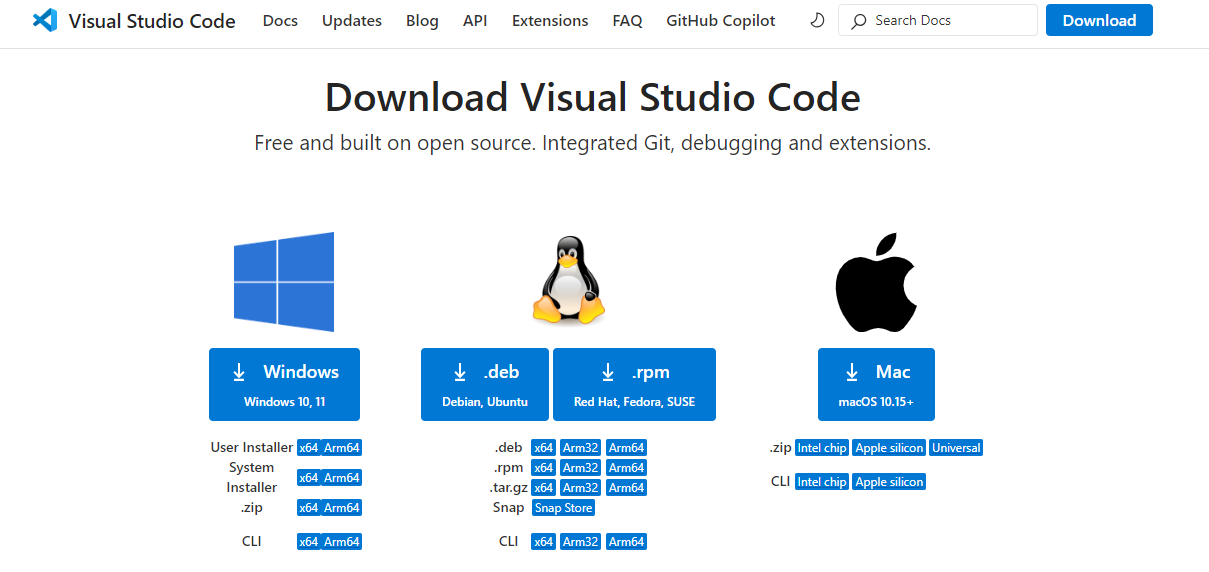
\includegraphics[scale =0.32]{img/vscode.png}
  \caption{Pantalla de instalación de Visual Studio Code. \textit{Elaboración propia.}}
  \label{fig:vscode_instalacion}
\end{figure}

  \item \textbf{Instalación de PlatformIO como extensión de VSCode:}
  \begin{itemize}
    \item Una vez abierto VSCode, hacer clic en el icono de extensiones (barra lateral izquierda).
    \item Buscar \texttt{PlatformIO IDE} y hacer clic en “Instalar”.
    \item Reiniciar VSCode tras la instalación para que la extensión se configure correctamente.
  \end{itemize}

  \begin{figure}[H]
  \centering
  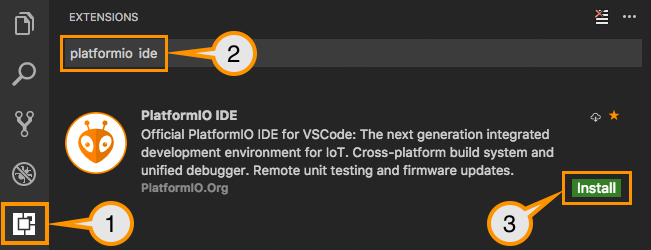
\includegraphics[width=0.65\textwidth]{img/platformio.png}
  \caption{Instalación de PlatformIO IDE desde el marketplace de Visual Studio Code. Fuente: \href{https://platformio.org/install/ide}{PlatformIO.}}
  \label{fig:platformio_instalacion}
\end{figure}

  \item \textbf{Instalación de Anaconda (incluye Python):}
  \begin{itemize}
    \item Descargar el instalador desde la página web de \href{https://www.anaconda.com/products/distribution}{Anaconda}.
    \item Seleccionar la versión para Windows e instalar con las opciones recomendadas.
    \item Anaconda incluye una instalación de Python, por lo que no es necesario instalarlo por separado.
  \end{itemize}

  \begin{figure}[H]
  \centering
  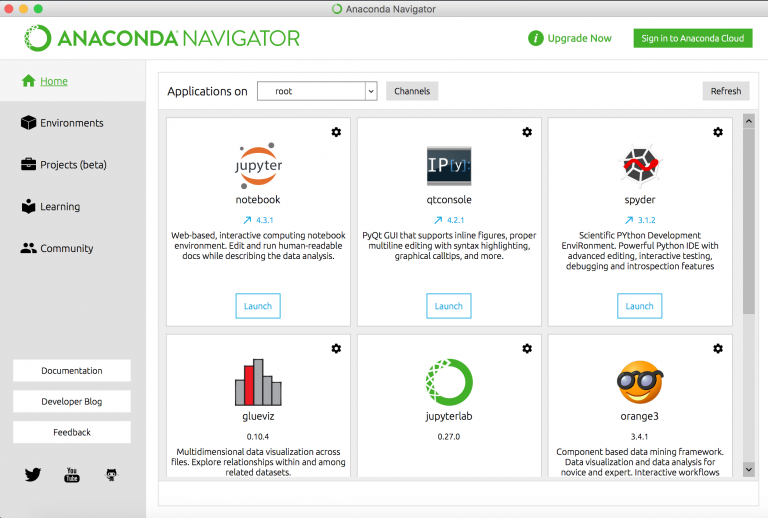
\includegraphics[width=0.65\textwidth]{img/anaconda-navigator.png}
  \caption{Instalación de Python desde Anaconda Navigator. Fuente: \href{https://www.aprendemachinelearning.com/instalar-ambiente-de-desarrollo-python-anaconda-para-aprendizaje-automatico/}{AprendeMachineLearning.}}
  \label{fig:anaconda_instalacion}
\end{figure}

  \item \textbf{Verificación de versiones de Python y Anaconda:}
  \begin{itemize}
    \item Abrir “Anaconda Prompt” y escribir:
    \begin{verbatim}
python --version
conda --version
    \end{verbatim}
    \item Deberían mostrarse las versiones instaladas. Las empleadas durante el desarrollo se recogen en la Tabla~\ref{tab:versiones_software}.
  \end{itemize}

  \item \textbf{Instalación de los drivers del programador EPS-Prog:}
  \begin{itemize}
    \item Es necesario instalar los drivers FTDI para que el programador sea reconocido como un puerto COM.
    \item Se puede seguir el tutorial oficial de \href{https://docs.platformio.org/en/stable/plus/debug-tools/esp-prog.html\#drivers}{PlatformIO.}
    \item Tras la instalación, el programador debe aparecer en el \textit{Administrador de dispositivos }de Windows bajo \textit{Puertos (COM y LPT)}.
    \item Para ello:
  \begin{itemize}
    \item Pulsar \texttt{Windows + R}, escribir \texttt{devmgmt.msc} y pulsar Enter o abrir directamente el \textit{Device Manager }desde el buscador de Windows.
    \item Desplegar el apartado \texttt{Puertos (COM y LPT)}.
    \item Debería aparecer una línea similar a \texttt{USB Serial Port (COM9)}.
  \end{itemize}
  \item Ese número de puerto (por ejemplo, \texttt{COM9}) será necesario para cargar el firmware, y en el caso de seguir esa metodología, para capturar datos con el script Python.
  \end{itemize}
\end{enumerate}

\subsection{Clonado y despliegue del firmware}

El código fuente original del firmware se encuentra disponible en el repositorio Git de la ONG, estructurado como un proyecto de PlatformIO. A continuación, se indican los pasos seguidos para clonar el proyecto, abrirlo en Visual Studio Code y cargarlo en la placa:

\begin{enumerate}
  \item \textbf{Clonado del repositorio:}
  \begin{itemize}
    \item Desde Visual Studio Code, abrir una nueva terminal.
    \item Ejecutar el comando:
    \begin{verbatim}
git clone https://github.com/medicalopenworld/in3ator.git
    \end{verbatim}
    \item También puede descargarse manualmente como archivo .zip y descomprimirse localmente\footnote{Dentro del repositorio, hacer click en el botón verde \texttt{Code} y seleccionar \texttt{Download ZIP}.}.
  \end{itemize}

  \item \textbf{Abrir el proyecto en PlatformIO:}
  \begin{itemize}
    \item Abrir VSCode y seleccionar la carpeta \texttt{Firmware/motherBoard}.
    \item PlatformIO detectará automáticamente el archivo \texttt{platformio.ini}, que define la configuración del proyecto.
    \item Verificar que la placa seleccionada sea la correcta (por ejemplo, ESP32) en dicho archivo.
  \end{itemize}

  \item \textbf{Compilación y carga del firmware:}
  \begin{itemize}
    \item Conectar la placa al ordenador mediante el programador EPS-Prog.
    \item Asegurarse de que el puerto COM detectado es el correcto.
    \item Desde la interfaz de PlatformIO (barra lateral izquierda), hacer clic en:
    \begin{itemize}
      \item \textbf{Build} (compilar el proyecto).
      \item \textbf{Upload} (cargar en el microcontrolador).
    \end{itemize}
    \item También puede hacerse desde terminal con:
    \begin{verbatim}
pio run --target upload
    \end{verbatim}
    \item Una vez cargado el firmware, se puede abrir el monitor serie desde PlatformIO (botón \textit{Monitor}) para verificar que la placa está enviando datos correctamente \footnote{Aunque el sensor no detecte el dedo, si el ordenador reconoce bien la placa, imprime los datos de las señales igualmente por la terminal.}.
  \end{itemize}
\end{enumerate} 

\subsection{Conexión del sistema físico}

Una vez instalado el entorno software y desplegado el firmware, el siguiente paso consiste en realizar las conexiones necesarias sobre la placa para que el sistema pueda funcionar correctamente y luego cargar el código que lee los datos. 

\textbf{Conectar la fuente de alimentación:}
  \begin{itemize}
    \item Utilizar una fuente de 12V con conector compatible.
    \item Conectarla a la entrada de alimentación de la PCB para suministrar energía al sistema.
  \end{itemize}

\textbf{Conectar el programador EPS-Prog:}
  \begin{itemize}
    \item Conectar el programador a la placa a través del cable JTAG a los pines correspondientes.
    \item Con un cable micro-USB, conectar el extremos micro-USB al programador y el extremo USB al ordenador. Una vez conectado, debería aparecer un nuevo puerto COM en el sistema.
  \end{itemize}

\textbf{Conectar el sensor óptico U401-D:}
  \begin{itemize}
    \item Conectar el sensor al conector designado en la placa.
    \item Asegurarse de que la orientación del conector sea correcta y que quede bien insertado.
  \end{itemize}


\section{Pruebas del sistema}
Para verificar el correcto funcionamiento del sistema completo, este apartado recoge las principales comprobaciones realizadas durante el desarrollo del sistema, para detectar posibles fallos en caso de que futuras personas retomen el proyecto y el sistema no funcione como se espera. 

Si tras seguir todos los pasos de instalación y despliegue, el sistema no responde correctamente, se recomienda revisar estos puntos para identificar en qué parte del proceso puede estar fallando.


\subsection{Comprobación del sensor óptico y alimentación de la placa}

Antes de acceder a los datos, lo primero que se debe comprobar es que el sensor óptico U401-D está correctamente conectado a la PCB y recibe alimentación. Al conectar la fuente de 12V, los LEDs del sensor deberían encenderse de forma visible. Si no se encienden aún estando conectado a la corriente eléctrica, pulsar el botón azul que se encuentra al reverso de la PCB.
\begin{figure}[H]
    \centering
    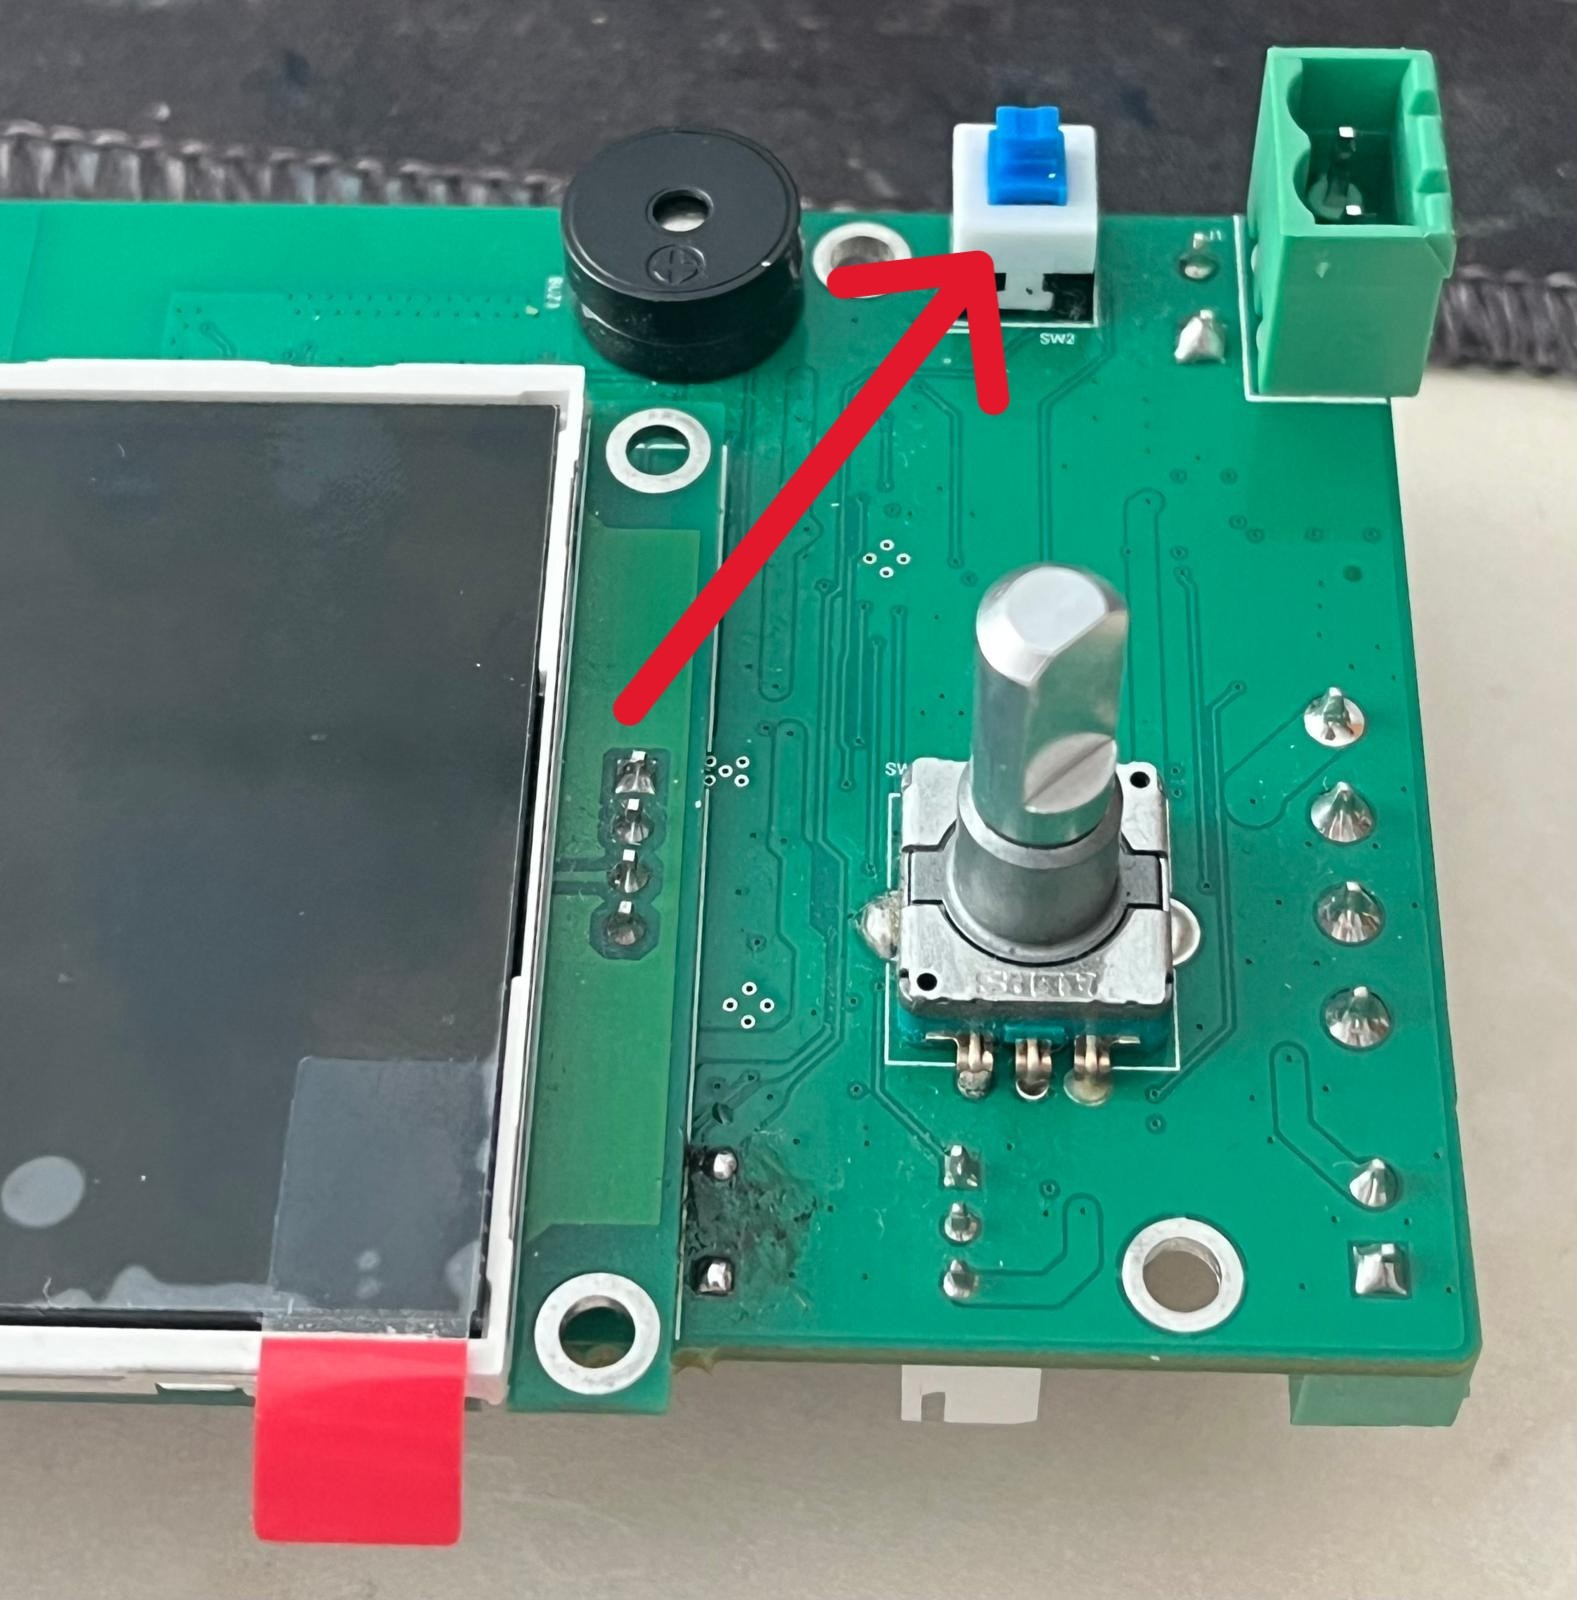
\includegraphics[width=0.5\linewidth]{img/boton.jpeg}
    \caption{Botón que enciende la placa si está apagada. \textit{Elaboración propia.}}
    \label{fig:botón}
\end{figure}
    
También es recomendable revisar que el conector esté orientado correctamente y bien insertado.

\subsection{Verificación de la comunicación por puerto serie}

Una vez asegurado que la placa está alimentada y que el sensor funciona, el siguiente paso es confirmar que el microcontrolador está enviando datos al ordenador a través del puerto serie. Esto puede comprobarse abriendo el monitor serie desde PlatformIO. 

Si el sistema está funcionando correctamente, al pulsar la opción \textit{Monitor} de PlatformIO deberían recibirse líneas con los valores crudos de los cuatro canales: IR, AMB\_IR, RED y AMB\_RED. Si no se recibe nada o aparecen símbolos extraños, puede ser que el puerto esté mal seleccionado o que el cable JTAG esté mal colocado.

Un aspecto importante a tener en cuenta es que el conector del programador puede colocarse de dos formas distintas, pero sólo es capaz de leer los datos en una de las posiciones. A continuación, se muestra la orientación correcta del cable plano sobre los pines de la placa. Es importante asegurarse de que la banda roja del cable queda alineada tal como se observa en la imagen \ref{fig: pines_prog}.

    \begin{figure}[H]
    \centering
    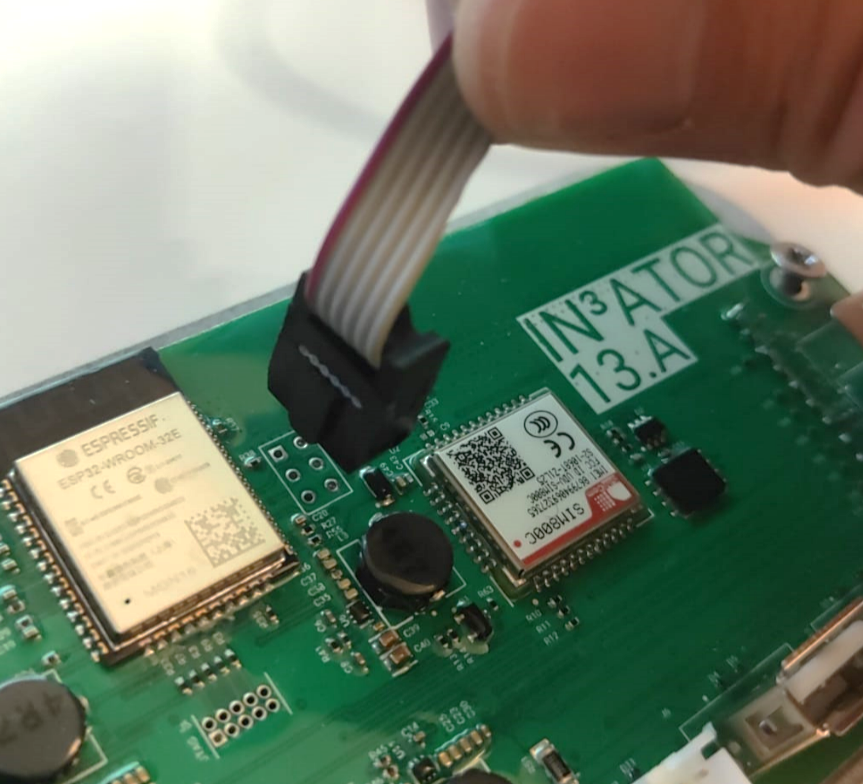
\includegraphics[width=0.5\textwidth]{img/pines_prog.png}
    \caption{Colocación correcta del cable del programador en la placa. \textit{Elaboración propia.}}
    \label{fig: pines_prog}
    \end{figure}

También es útil revisar en el Administrador de dispositivos (Windows) para ver si el programador EPS-Prog ha sido detectado como puerto COM. Si no aparece, el problema puede estar en los drivers FTDI o en la conexión física del programador.

\begin{figure}[H]
  \centering
  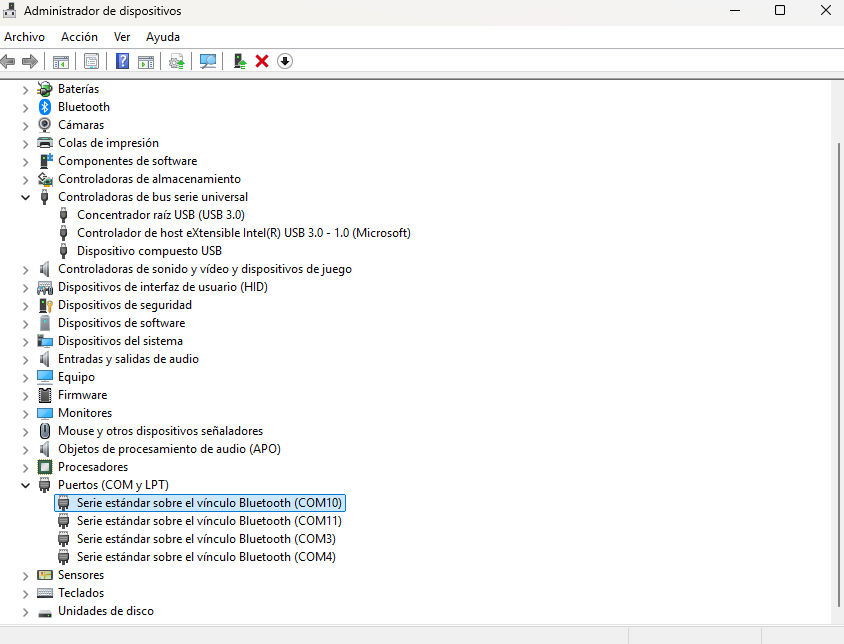
\includegraphics[width=0.85\textwidth]{img/device_manager.png}
  \caption{Interfaz del Device Manager de Windows \textbf{sin} el programador conectado.}
  \label{fig:device_manager}
\end{figure}

\begin{figure}[H]
  \centering
  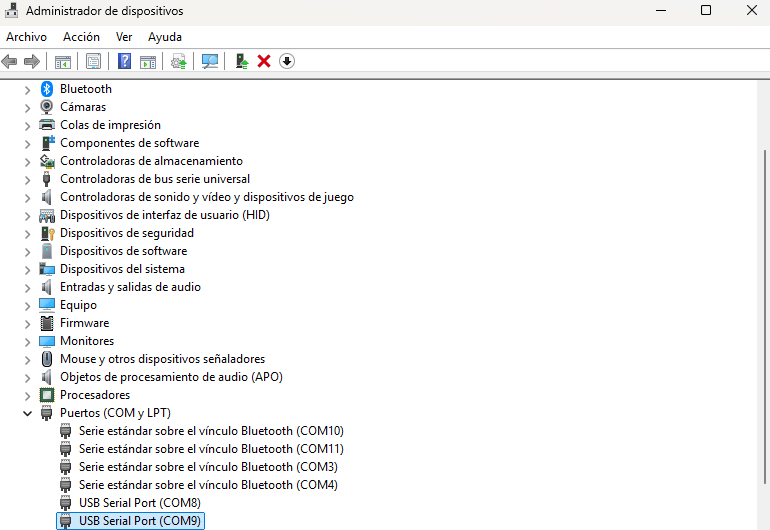
\includegraphics[width=0.85\textwidth]{img/device_manager2.png}
  \caption{Interfaz del Device Manager de Windows \textbf{con} el programador conectado.}
  \label{fig:device_manager2}
\end{figure}


\subsection{Alternativa de trabajo basada en archivos CSV}

En el caso de que se quieran validar los algoritmos directamente sobre el microcontrolador, se pueden recopilar en archivos .csv para analizarlos en Jupyter Notebook. Para seguir este enfoque y continuar haciendo pruebas adicionales a las presentadas, se recomienda utilizar el siguiente procedimiento:

Desde el firmware \textbf{original} del proyecto, intercambiar la función denominada \texttt{get\_AFE44XX\_Data}\footnote{Esta función modificada se encuentra dentro del directorio \texttt{Código.}} por la función modificada disponible en el repositorio de este TFG \footnote{\href{https://github.com/ElenaRuizMoreno/TFG-Elena-Ruiz/}{TFG-ElenaRuiz}}. Cargar el código en VSCode (mediante \textit{Upload} de PlatformIO) con los cambios realizados. Si se ha subido correctamente, tiene que aparecer lo siguiente:

\begin{figure}[H]
    \centering
    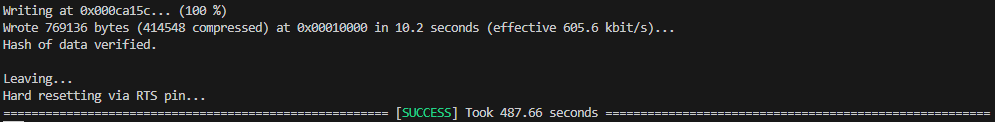
\includegraphics[scale=0.5]{img/succes.png}
    \caption{Mensaje que aparece al haber cargado el firmware correctamente en la PCB.}
    \label{fig:success}
\end{figure}


Descargar del repositorio el script \texttt{save\_log2.py}\footnote{El archivo se encuentra en el directorio \textit{procesamiento}, dentro del directorio principal \textit{Código}}. Este código lo que hace es leer datos desde la PCB conectada por puerto serie y guardarlos en un archivo CSV con una duración de 30 segundos y con las cabeceras correspondientes de cada columna. Para ello, hay que configurar tres cosas:

\begin{itemize}
    \item \texttt{SERIAL\_PORT = ``COMX"}: Define el puerto serie donde está conectada la PCB (comprobar a través del \textit{Device Manager} o PlatformIO)
    \item \texttt{BAUD\_RATE = 115200}: Establece la velocidad de transmisión de datos (115200 baudios), que debe coincidir con la del firmware de la placa\footnote{Este valor se puede encontrar dentro del archivo \texttt{platformio.ini} del proyecto, correspondiente a la variable \texttt{monitor\_speed}}.
    \item \texttt{OUTPUT\_FILE}: Especifica la ruta y nombre del archivo donde se guardarán los datos CSV. Cambiar según donde se quiera almacenar.
\end{itemize}

Una vez configuradas estas especificaciones, ejecutar el fichero en el Prompt de \textit{Anaconda} con el comando \texttt{python save\_log2.py} en la ruta del directorio donde esté ubicado. A la vez que se ejecuta, el sensor debe estar colocado en el dedo evitando exceso de luz o movimiento durante los segundos que dura cada registro. 

Es importante comprobar que los archivos generados contienen las columnas esperadas y que los valores cambian con el tiempo (es decir, que no son todos ceros o constantes). Si el archivo está vacío o con líneas incompletas, puede deberse a errores de lectura, desconexiones intermitentes o saturación del buffer serie.

\section{Instrucciones para la modificación o mejora del proyecto.}

Con el fin de ampliar o adaptar el sistema actual, a continuación, se describen los elementos del código y del hardware que se deben tener en cuenta para realizar cambios o implementar mejoras.

En cuanto al hardware y sus conexiones físicas, es importante tener en cuenta que el sistema ha sido desarrollado utilizando el material facilitado por la ONG Medicina Abierta al Mundo. Los componentes mencionados son los que se prevé utilizar en caso de que el proyecto se consolide y pase a emplearse de forma real en las incubadoras. Por tanto, no se recomienda modificar ni sustituir estos elementos, ni alterar su forma de conexión, ya que el diseño actual responde a limitaciones de coste y criterios de disponibilidad y compatibilidad definidos por la organización. 

\subsection{Modificación de algoritmos de procesamiento}

Los algoritmos de estimación de frecuencia cardíaca y SpO$_2$ se encuentran implementados inicialmente en formato notebook (\texttt{procesamiento/}) para su validación sobre datos en CSV. En caso de querer incluir nuevos algoritmos y estimaciones para después llevarlo al firmware, se recomienda:

\begin{itemize}
    \item Validar el nuevo algoritmo primero en Jupyter Notebook.
    \item Extraer las funciones clave y convertirlas a C++.
    \item Sustituir las funciones dentro de las funciones \texttt{spo2\_algorithm.cpp} y/o \texttt{hr\_estimation.cpp} según corresponda.
\end{itemize}

\subsection{Ajuste de parámetros de adquisición}

En el archivo \texttt{platformio.ini}, es posible modificar:

\begin{itemize}
    \item \texttt{monitor\_speed}: velocidad de transmisión por puerto serie.
    \item \texttt{build\_flags}: definición de macros para configurar el comportamiento del firmware.
\end{itemize}

Dentro del código fuente, pueden ajustarse:

\begin{itemize}
    \item Tiempo de adquisición por registro.
    \item Frecuencia de muestreo.
    \item Umbrales de detección de picos.
\end{itemize}

\subsection{Ampliación de funcionalidades}

Algunas ideas de ampliación que pueden llevarse a cabo directamente sobre la base del código existente:

\begin{itemize}
    \item Añadir visualización gráfica de la señal en la pantalla TFT (requiere librerías gráficas).
    \item Guardar registros en una tarjeta SD o memoria interna.
    \item Implementar conexión Bluetooth para enviar los datos a una app externa.
\end{itemize}
\apendice{Descripción de adquisición y tratamiento de datos}
Como se mencionó en la memoria de este proyecto, se han generado datos experimentales propios a partir del sistema de adquisición implementado. No se ha recurrido al uso de bases de datos públicas o registros externos. Para ello, se ha desarrollado un sistema de adquisición personalizado, orientado a la captura de señales fotopletismográficas en distintas condiciones.

\section{Descripción formal de los datos}

Los datos registrados durante el proyecto se almacenan en ficheros CSV, generados automáticamente y en tiempo real por el microcontrolador del sistema a partir de los valores recogidos por el sensor óptico U401-D, gobernado por el chip AFE4490. El proceso de adquisición de los datos fue descrito en la sección de la \textit{Metodología} de la memoria del trabajo.
Cada fichero corresponde a una sesión de adquisición de aproximadamente 30 segundos de duración, con una frecuencia de muestreo cercana a 60 Hz.

El archivo contiene cinco columnas, cuyas variables y rangos observados son:

\begin{itemize}
  \item \textbf{Tiempo (ms)}: Marca temporal de la muestra, iniciando en 0 ms y finalizado el registro en 30 000 ms. Permite reconstruir la señal en el dominio temporal. Los logs tienen esta duración para poder limpiar la señal y tener un rango de valores lo suficientemente extenso como para no perder información y poder analizar los datos de una manera válida.
  
  \item \textbf{IR}: Señal óptica infrarroja medida con el LED de 940 nm encendido. Se utiliza para el análisis de la variabilidad pulsátil del volumen sanguíneo (frecuencia cardíaca) y estimación de SpO\textsubscript{2}. La señal varía cíclicamente con el pulso, reflejando los latidos del corazón.
  
  \item \textbf{AMB\_IR}: Nivel de luz infrarroja ambiente medida con el LED apagado.  Sirve para estimar y corregir la interferencia ambiental en la señal IR. Es útil para eliminar el ruido proveniente de fuentes de luz externas (como luz artificial, luz solar, etc.). Se resta de la señal IR para obtener solo la parte útil emitida por el LED.
  
  \item \textbf{RED}: Señal óptica roja con el LED de 660 nm encendido. La absorción de luz roja varía según el nivel de oxígeno en la sangre. También varía con el pulso, pero de forma distinta a la señal IR.
  
  \item \textbf{AMB\_RED}: Representa la medición de luz roja captada con LED rojo apagado, es decir, la luz ambiental en la misma longitud de onda. Igual que AMB\_IR, se utiliza para corregir la señal RED restando la componente ambiental.

\end{itemize}

\begin{figure}[H]
    \centering
    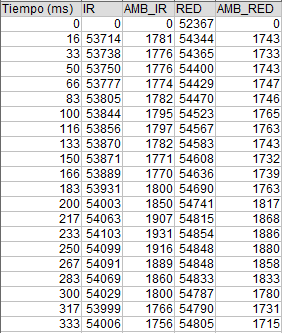
\includegraphics[scale=0.80]{img/Datos crudos csv.png}
    \caption{Ejemplo de unos milisegundos de un registro de datos crudos. \textit{Elaboración propia.}}
    \label{fig:datos_crudos}
\end{figure}

\newpage

Para cada longitud de onda (IR y RED), se realiza:
\begin{itemize}
    \item \texttt{IR\_real = IR - AMB\_IR}
    \item \texttt{RED\_real = RED - AMB\_RED}
\end{itemize}

Esto permite obtener solo la señal útil (emitida por el LED y absorbida por el tejido), eliminando el ruido ambiental. Las señales corregidas se usan luego para detectar picos y calcular el cociente de absorción IR/RED.

\subsection{Rango y unidades de las señales}

Los valores registrados en las columnas \texttt{IR}, \texttt{RED}, \texttt{AMB\_IR} y \texttt{AMB\_RED} no están expresados en unidades físicas como voltios o miliwatios, sino que corresponden a valores crudos digitalizados, generados por el convertidor ADC interno del circuito AFE4490.

Este ADC tiene una resolución de 22 bits con signo, por lo que puede generar un amplio intervalo de valores. Sin embargo, en las configuraciones utilizadas en este proyecto, los valores reales registrados caen dentro de los siguientes rangos típicos:

\begin{itemize}
    \item \textbf{IR}: 30.000 – 65.000 unidades. Señal infrarroja útil, más estable que la roja.
    \item \textbf{RED}: 3.000 – 65.000 unidades. Señal roja, con mayor dispersión entre sesiones.
    \item \textbf{AMB\_IR} y \textbf{AMB\_RED}: 0 – 10.000 unidades. Corresponden a luz ambiental; idealmente deberían ser bajas.
\end{itemize}

Aunque no se cuenta con una calibración para traducir estos valores a magnitudes físicas, su uso es  válido para el análisis de la señal pulsátil y la posterior estimación de parámetros fisiológicos.


\subsection{Análisis de tendencias}

Inicialmente se planteó la hipótesis de que una frecuencia cardíaca más baja estaría asociada a valores medios de señal más altos (por ejemplo, debido a mayor volumen sistólico o perfusión). Sin embargo, el análisis de varios registros no ha mostrado una correlación directa ni consistente entre la frecuencia cardíaca y el valor medio de las señales IR o RED.

Esta variabilidad puede explicarse por múltiples factores, entre ellos:

\begin{itemize}
    \item Diferencias en la presión de colocación del sensor.
    \item Cambios en la perfusión periférica o temperatura de los dedos.
    \item Ruido de fondo e interferencias ópticas del entorno.
    \item Distintas configuraciones del AFE4490 durante las sesiones.
\end{itemize}

Por tanto, el sistema se basa exclusivamente en la relación relativa entre componentes de cada señal y no en su valor absoluto.

\subsection{Alamacenamiento de los datos}

Los archivos se nombran con el formato:

\begin{center}
  \texttt{raw\_data\_\{SpO2\}\_\{HR\}.csv}
\end{center}

donde \texttt{\{SpO2\}} y \texttt{\{HR\}} representan los valores de saturación de oxígeno y frecuencia cardíaca registrados simultáneamente en otro dedo del usuario por un par de pulsioxímetros comerciales externos para validación cruzada. Gracias a la referencia de ambos valores a través del nombre del archivo, se puede validar el valor que se obtiene en la estimación del código.

Los ficheros están clasificados por:

\begin{itemize}
  \item \textbf{Calidad de la señal}: buena o mala.
  \item \textbf{Condición fisiológica del sujeto}: reposo, post-ejercicio, apnea breve, iluminación variable.
\end{itemize}

\section{Descripción clínica de los datos}

Aunque algunos de los conceptos presentados en esta sección ya han sido explicados previamente en el capítulo de fundamentos teóricos, se recogen aquí de forma resumida y aplicada al contexto experimental, de acuerdo con los objetivos específicos de este anexo.


La señal adquirida es una señal PPG, obtenida mediante iluminación del tejido con luz en dos longitudes de onda: infrarrojo (940 nm) y rojo (660 nm). La absorción de la luz depende del contenido de hemoglobina oxigenada y desoxigenada en sangre. La señal resultante tiene dos componentes:

\begin{itemize}
  \item \textbf{Componente DC}: relacionada con tejidos estáticos y sangre no pulsátil.
  \item \textbf{Componente AC}: refleja el pulso arterial y permite detectar la frecuencia cardíaca.
\end{itemize}

Los parámetros fisiológicos que pueden ser extraídos con estos datos son la frecuencia cardíaca y la saturación de oxígeno.

Los datos fueron adquiridos con un sujeto sano adulto bajo diferentes condiciones simuladas:

\begin{itemize}
  \item \textbf{Reposo absoluto}: señal estable, sin interferencias.
  \item \textbf{Post-ejercicio}: incremento de HR y aparición de ruido.
  \item \textbf{Apnea breve}: reducción inducida de SpO\textsubscript{2}.
  \item \textbf{Iluminación variable}: para evaluar la robustez ante interferencia lumínica.
\end{itemize}

Las señales ambientales (\texttt{AMB\_IR} y \texttt{AMB\_RED}) permiten compensar adecuadamente la luz del entorno para mantener la precisión en escenarios reales. Además, se identificaron registros inválidos debido a movimientos, baja perfusión o problemas de contacto, los cuales no fueron eliminados sino clasificados para evaluar el rendimiento del algoritmo en situaciones adversas.

Cuando los datos adquiridos en formato \texttt{.csv} se representan gráficamente en el dominio temporal, se obtiene una señal como la que se muestra a continuación:

\begin{figure}[H]
    \centering
    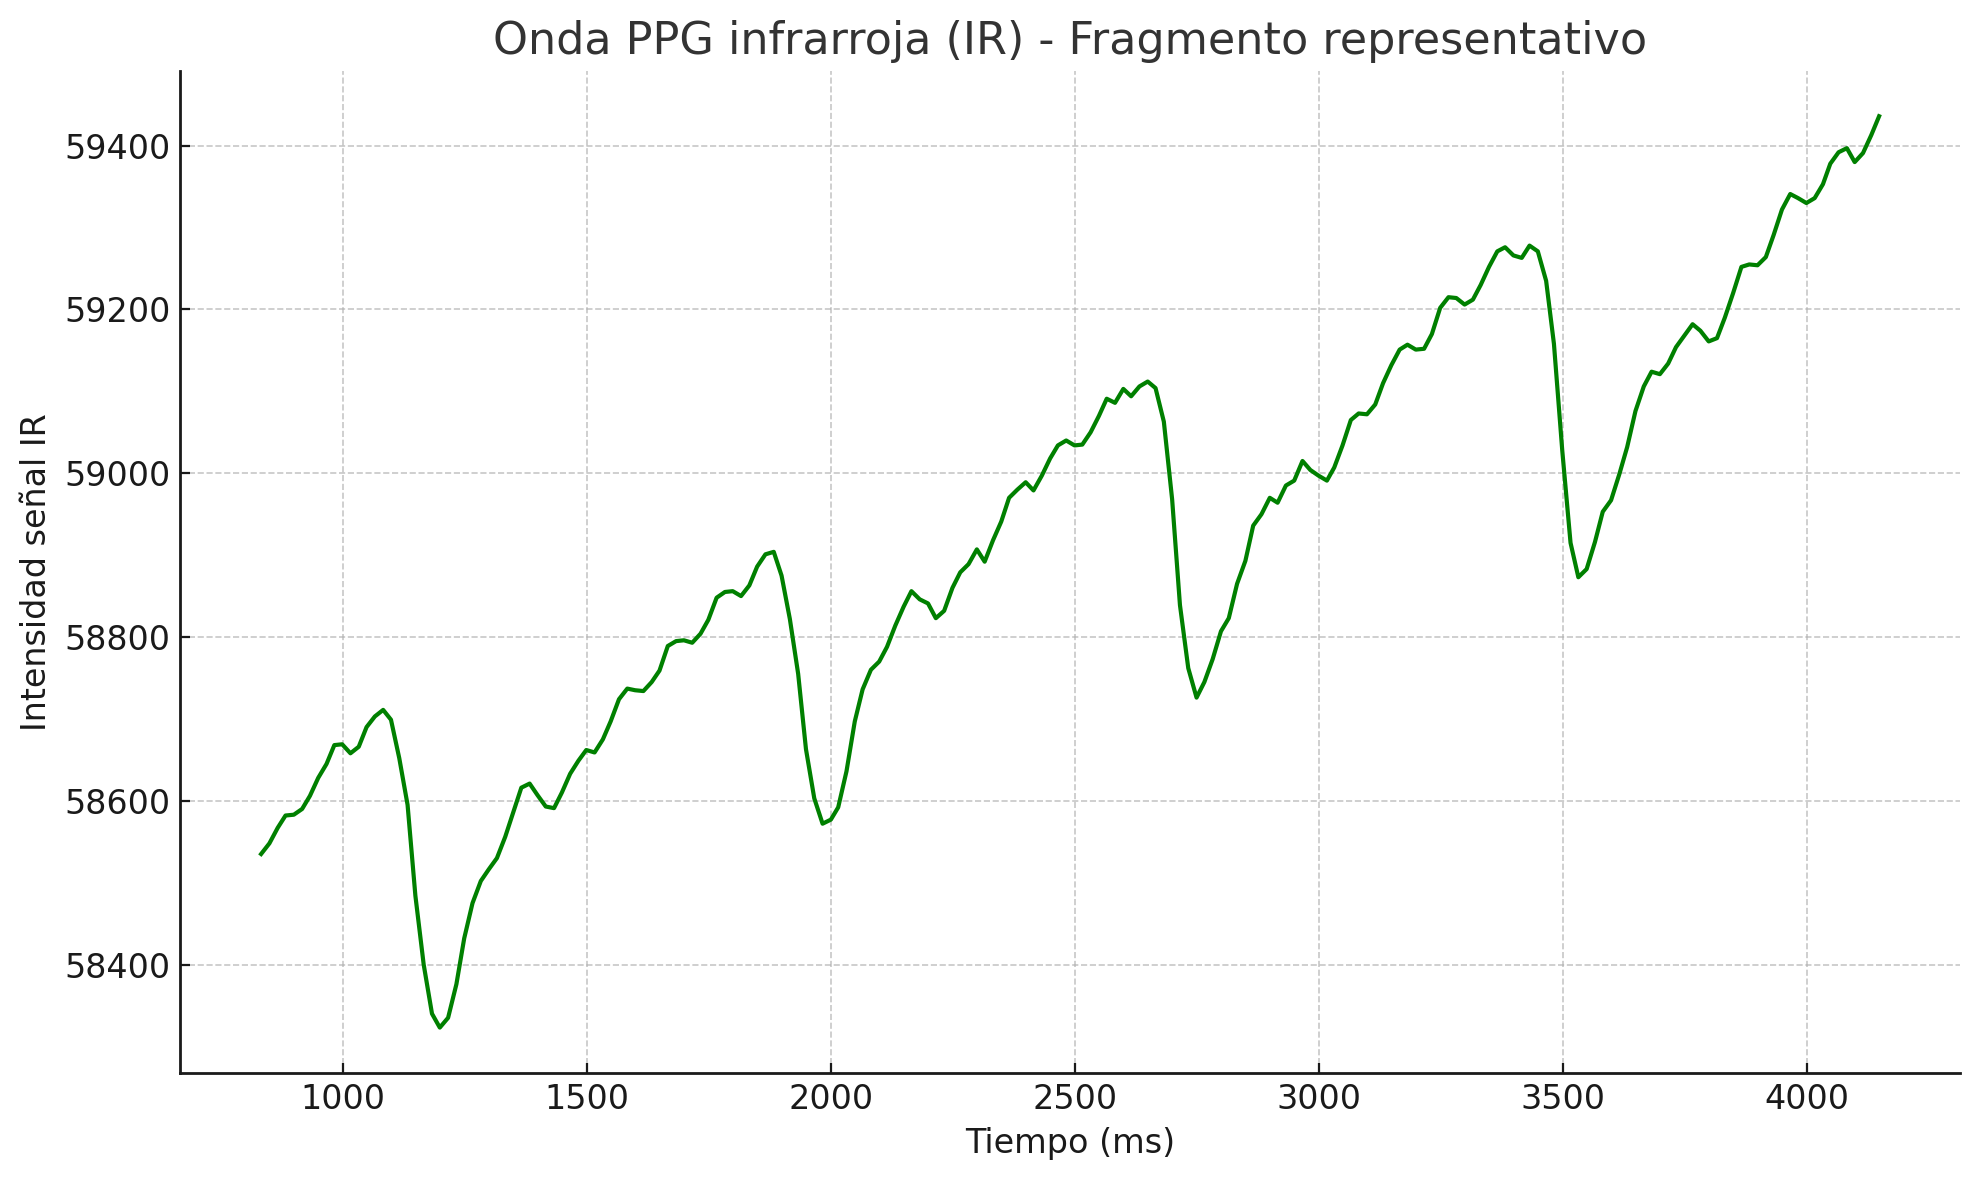
\includegraphics[width=0.95\linewidth]{img/forma_onda_PPG.png}
    \caption{Onda PPG del canal IR. El fragmento muestra aproximadamente 6 pulsos cardíacos completos correspondientes a un registro con HR = 69 bpm. \textit{Elaboración propia.}}
    \label{fig:ppg_morfologia}
\end{figure}

La señal PPG presenta una estructura morfológica característica que refleja directamente los cambios en el volumen sanguíneo arterial. Como se muestra en la Figura~\ref{fig:ppg_partes}, la señal está compuesta por:

\begin{itemize}
    \item \textbf{Pico primario (primary peak)}: punto máximo de cada ciclo, asociado a la presión máxima durante la sístole.
    \item \textbf{Trough}: punto mínimo del ciclo, justo antes del ascenso del siguiente pulso. Se utiliza como referencia para medir la amplitud.
    \item \textbf{Pulse amplitude}: diferencia entre el pico sistólico y el trough. Representa la magnitud del componente pulsátil AC.
    \item \textbf{Pulse width}: duración temporal del ciclo, medida como el tiempo entre dos picos consecutivos. Está relacionada con el intervalo RR y, por tanto, con la frecuencia cardíaca.
    \item \textbf{Pico secundario o muesca dicrota (secondary peak)}: pequeña inflexión o repunte que aparece en la fase de descenso, visible en señales de alta calidad, asociada al cierre de la válvula aórtica.
\end{itemize}

\begin{figure}[H]
    \centering
    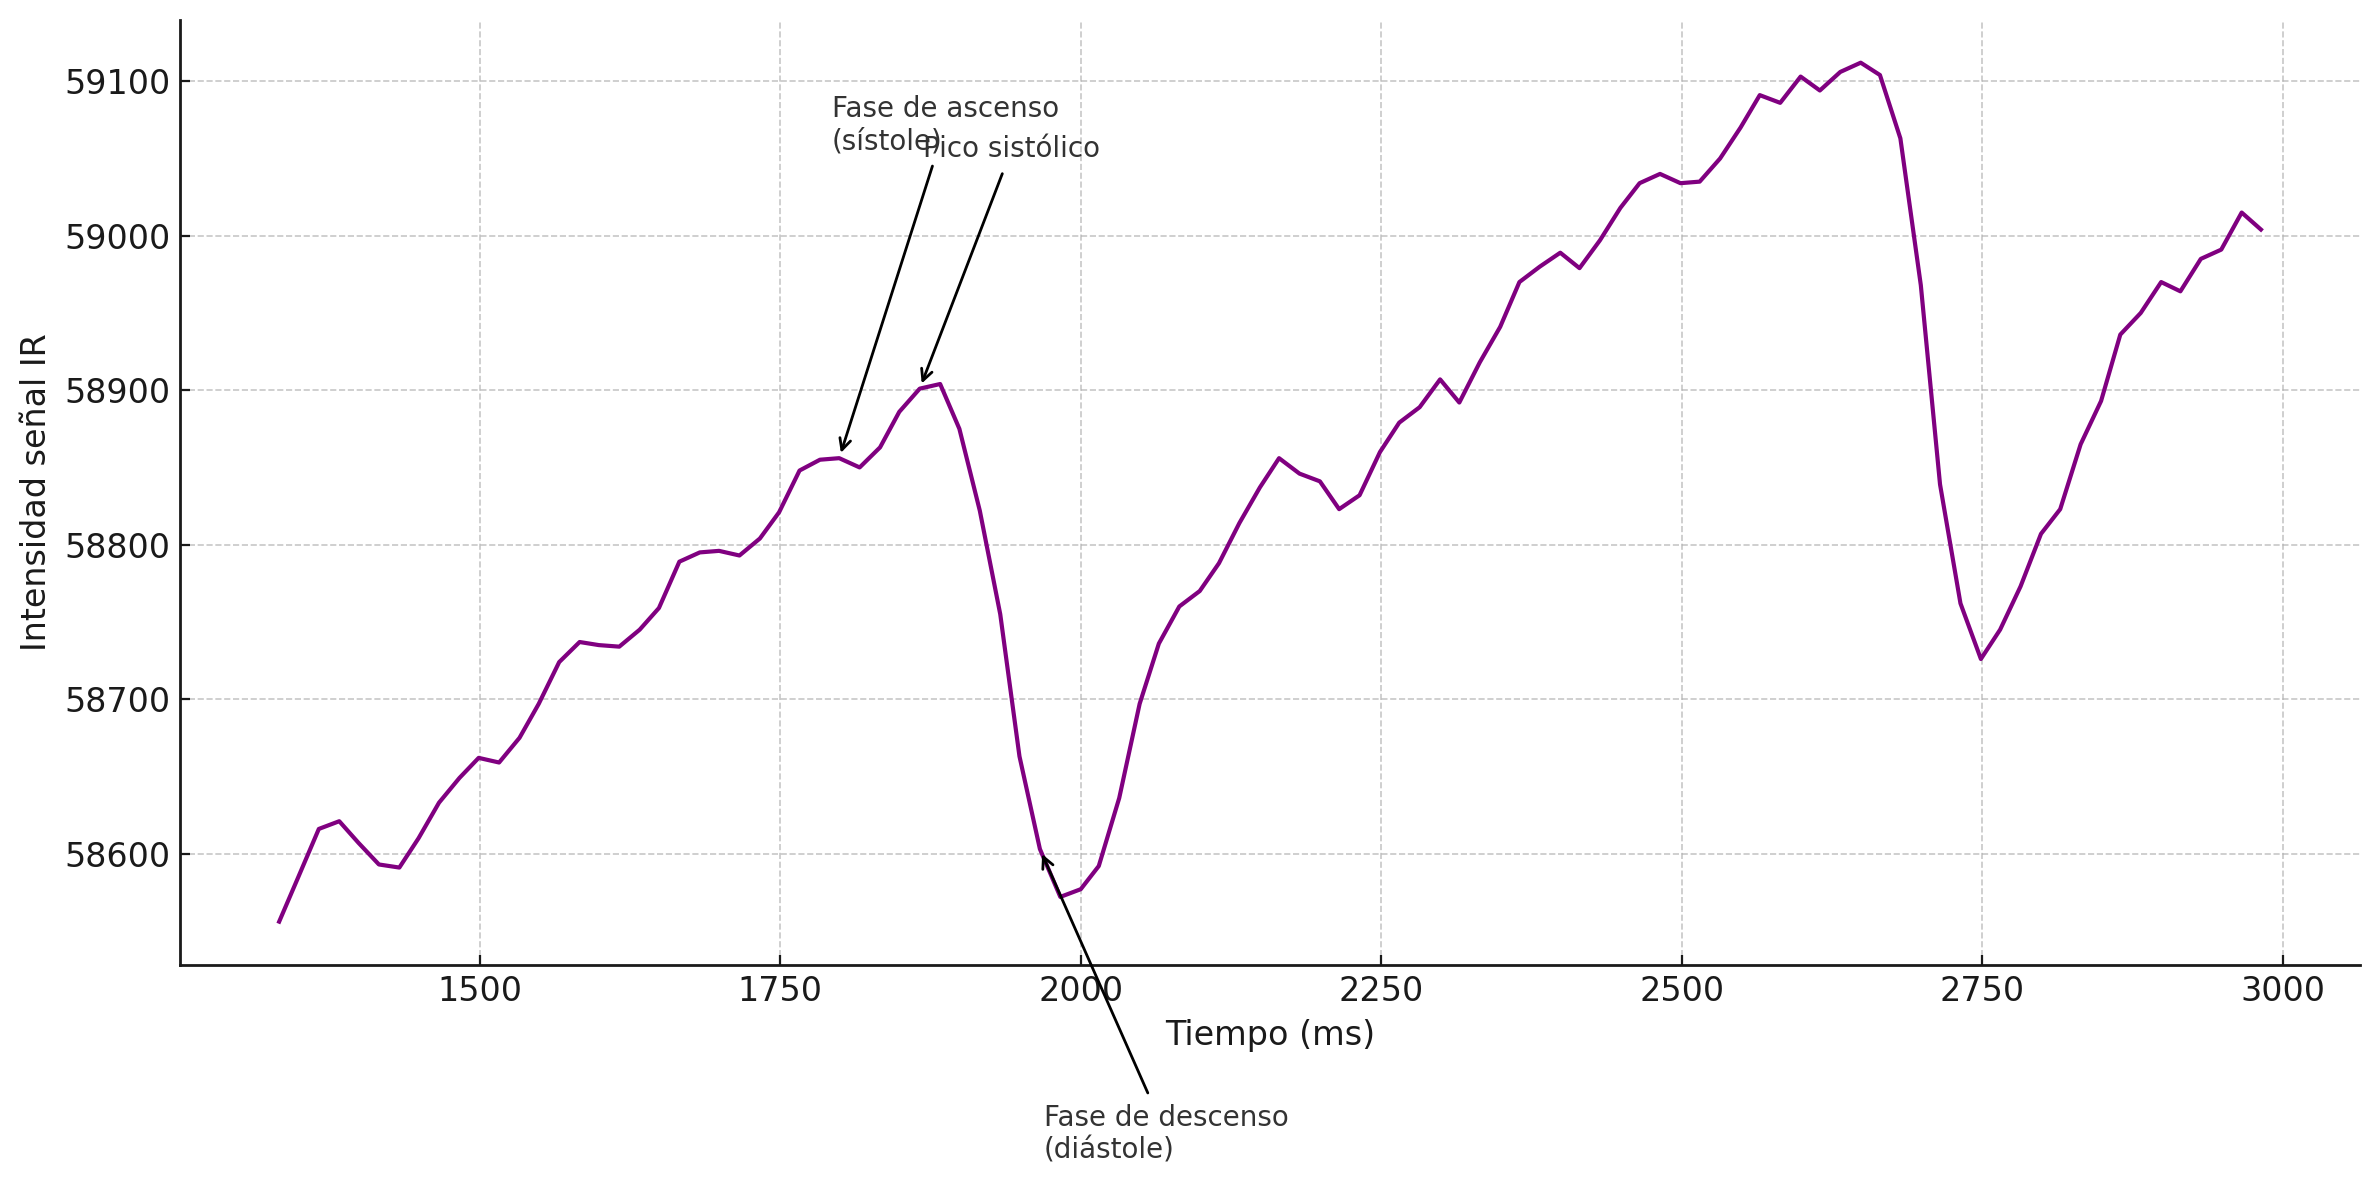
\includegraphics[width=1\linewidth]{img/partesPPG.png}
    \caption{Detalle ampliado de la señal PPG. Se muestran dos pulsos cardíacos completos y se anotan las fases principales de la morfología. Fuente: \cite{oximetria_medium}.}
    \label{fig:ppg_partes}
\end{figure}

Una forma de saber si los datos son válidos para su posterior análisis, es graficar las señales para comprobar que la morfología sea claramente visible y así garantizar una interpretación clínica aceptable. La correcta identificación de los picos es necesaria para el cálculo de la frecuencia cardíaca, y la forma general de la señal (incluyendo su amplitud relativa y periodicidad) afecta directamente a la estimación de la saturación de oxígeno. 

No es indispensable que la señal se comporte de esta manera a lo largo de todo el período que dure la medición, pero sí que es importante que durante unos segundos se mantenga esta estructura para poder identificar los picos necesarios para hacer el cálculo.

El tratamiento posterior de los datos se llevó a cabo en \texttt{Python} mediante entornos de trabajo \texttt{Jupyter Notebook}, donde se aplicaron algoritmos de filtrado digital, detección de picos y cálculo de estimaciones agregadas de SpO\textsubscript{2} y frecuencia cardíaca. Los valores obtenidos se compararon con las medidas externas para evaluar la precisión del sistema.



\apendice{Manual de especificación de diseño}

A continuación, se presenta el diseño técnico del sistema de pulsioximetría desarrollado, incluyendo los esquemas eléctricos más relevantes y los diagramas de bloques de los algoritmos utilizados, con el objetivo de dejar documentada la arquitectura general tanto a nivel de hardware como de procesamiento de señal. 

Dado que el desarrollo se ha realizado a partir de material previamente existente, se ha incluido una sección que contextualiza el estado del sistema antes del inicio del trabajo, detallando los recursos existentes proporcionados por el equipo de \textit{In$^3$ator} sobre los que se ha construido esta implementación.

\section{Punto de partida}

El presente trabajo parte de una base sólida ya desarrollada por el equipo de la ONG Medicina Abierta al Mundo, responsable del diseño, fabricación y distribución de la incubadora de bajo coste \textit{In$^3$ator} (figura \ref{fig:in3ator23}). 

Esta incubadora, que ha sido puesta en funcionamiento en países con recursos limitados, cuenta con un sistema electrónico y de control completamente operativo, cuyo diseño de hardware y firmware cubre funciones esenciales como la regulación de temperatura, humedad, ventilación, fototerapia y alarmas de seguridad.

\begin{figure}[H]
    \centering
    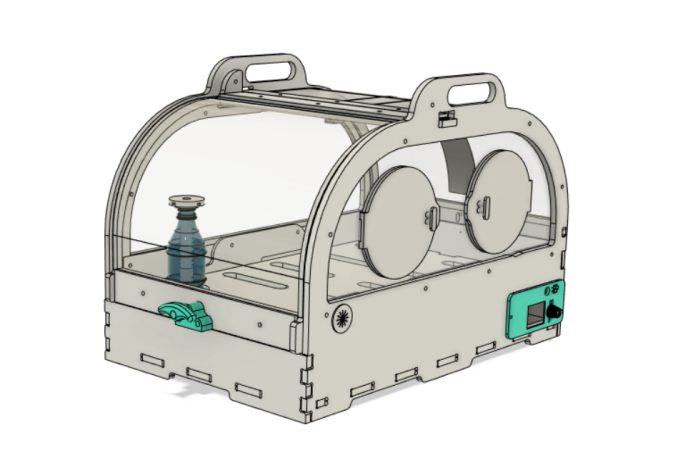
\includegraphics[width=0.75\linewidth]{img/in3ator23.png}
    \caption{Diseño 3D de la incubadora neonatal \textit{In$^3$ator} version 2.1. Fuente: \cite{in3ator2023manual}.}
    \label{fig:in3ator23}
\end{figure}

Actualmente, las incubadoras distribuidas por la ONG no cuentan con funcionalidad de pulsioximetría integrada. Sin embargo, con el objetivo de investigar su posible implementación, el equipo de \textit{In$^3$ator} incorporó de forma experimental esta funcionalidad en el hardware (figura \ref{fig:PCB2}) de un prototipo. Este sistema nos fue cedido para el desarrollo y validación del algoritmo correspondiente. La placa electrónica ya disponía de un sistema de adquisición basado en el AFE4490, así como de una interfaz con el microcontrolador ESP32. 

\begin{figure}[H]
    \centering
    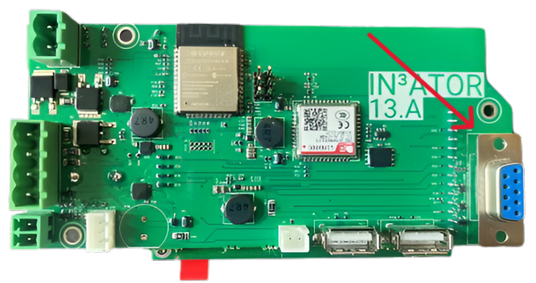
\includegraphics[width=0.75\linewidth]{img/PCB2.png}
    \caption{Placa electrónica modificada con la funcionalidad de pulsioximetría integrada. Fuente: \textit{Elaboración propia}.}
    \label{fig:PCB2}
\end{figure}

El firmware general del sistema estaba también desarrollado, con una estructura que permitía incorporar nuevas funciones. Dentro de este contexto, mi trabajo se ha centrado en el archivo \texttt{SPO2.cpp} (\ref{fig:firmware}), donde he implementado, por una parte, la función que extraía los datos crudos del sensor para poder estudiar los procedimientos por separado; y por otra, el algoritmo de estimación de frecuencia cardíaca y saturación de oxígeno a partir de las señales obtenidas por el sensor óptico en tiempo real.

\begin{figure}[H]
    \centering
    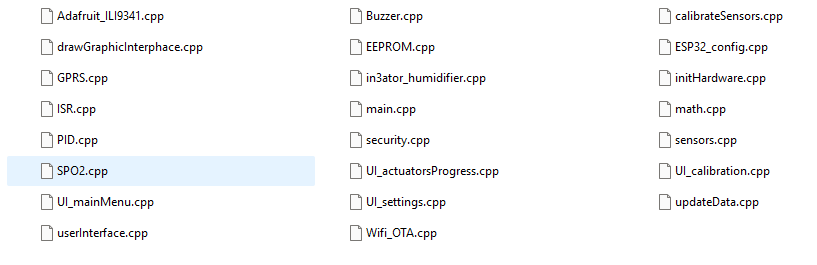
\includegraphics[width=1\linewidth]{img/firmware.png}
    \caption{Estructura de archivos del directorio \texttt{src/}del firmware original. \textit{Elaboración propia}.}
    \label{fig:firmware}
\end{figure}

Para desarrollar estos algoritmos, se realizó primero un estudio experimental en Python a través de Jupyter Notebooks, partiendo desde cero, basándome en artículos científicos y documentos técnicos, como los proporcionados por fabricantes de sensores comerciales (por ejemplo, OB1203). A partir de estos análisis, se seleccionaron los métodos más adecuados para su implementación en el entorno embebido del ESP32.

En cuanto a la integración hardware, no fue necesario modificar la placa, ya que era completamente funcional. Mi labor consistió en aprender a conectarla correctamente, instalar los drivers necesarios y adquirir pulsioxímetros comerciales como referencia externa para validar los resultados obtenidos por el sistema. Para ello, se nos proporcionaron los planos correspondientes a la estructura electrónica de la placa donde se podía observar con detalle la disposición de los componentes relevantes para la funcionalidad de pulsioximetría. Estos planos se analizan a continuación con el objetivo de contextualizar el entorno hardware sobre el que se desarrolló este proyecto.

\newpage

\section{Planos}

En esta sección se recogen los esquemas eléctricos relacionados con el subsistema de pulsioximetría implementado en este trabajo. Los planos han sido extraídos de los esquemáticos completos \footnote{Accesibles desde GitHub, dentro del directorio principal de \texttt{Documentación de referencia}} proporcionados por el equipo de desarrollo del proyecto \textit{In$^3$ator}, centrándose exclusivamente en los componentes que intervienen en la adquisición y transmisión de las señales fotopletismográficas.

La implementación se basa en tres bloques:
\begin{itemize}
    \item El \textbf{AFE4490}, un circuito especializado que capta y digitaliza la señal óptica procedente del sensor de pulsioximetría.
    \item El \textbf{sistema de alimentación}, que permite el funcionamiento autónomo mediante batería y gestiona la distribución de voltajes adecuados a cada componente.
    \item El \textbf{microcontrolador ESP32}, que ejecuta el firmware encargado de controlar el sensor, procesar las señales y enviar los datos.
\end{itemize}

A continuación se muestran los esquemas correspondientes, cada uno acompañado de una breve descripción técnica que resume su funcionalidad dentro del sistema.
\subsection{Circuito de adquisición AFE4490}

Este circuito es el encargado de recibir la se\~nal \'optica captada por el sensor (LED y fotodiodo), amplificarla, filtrarla y convertirla a formato digital. Aunque el esquema incluye muchos componentes, lo m\'as relevante para este proyecto es identificar el chip AFE4490, las entradas de se\~nal, y las conexiones SPI que permiten que el microcontrolador reciba los datos digitalizados.

\begin{figure}[H]
\centering
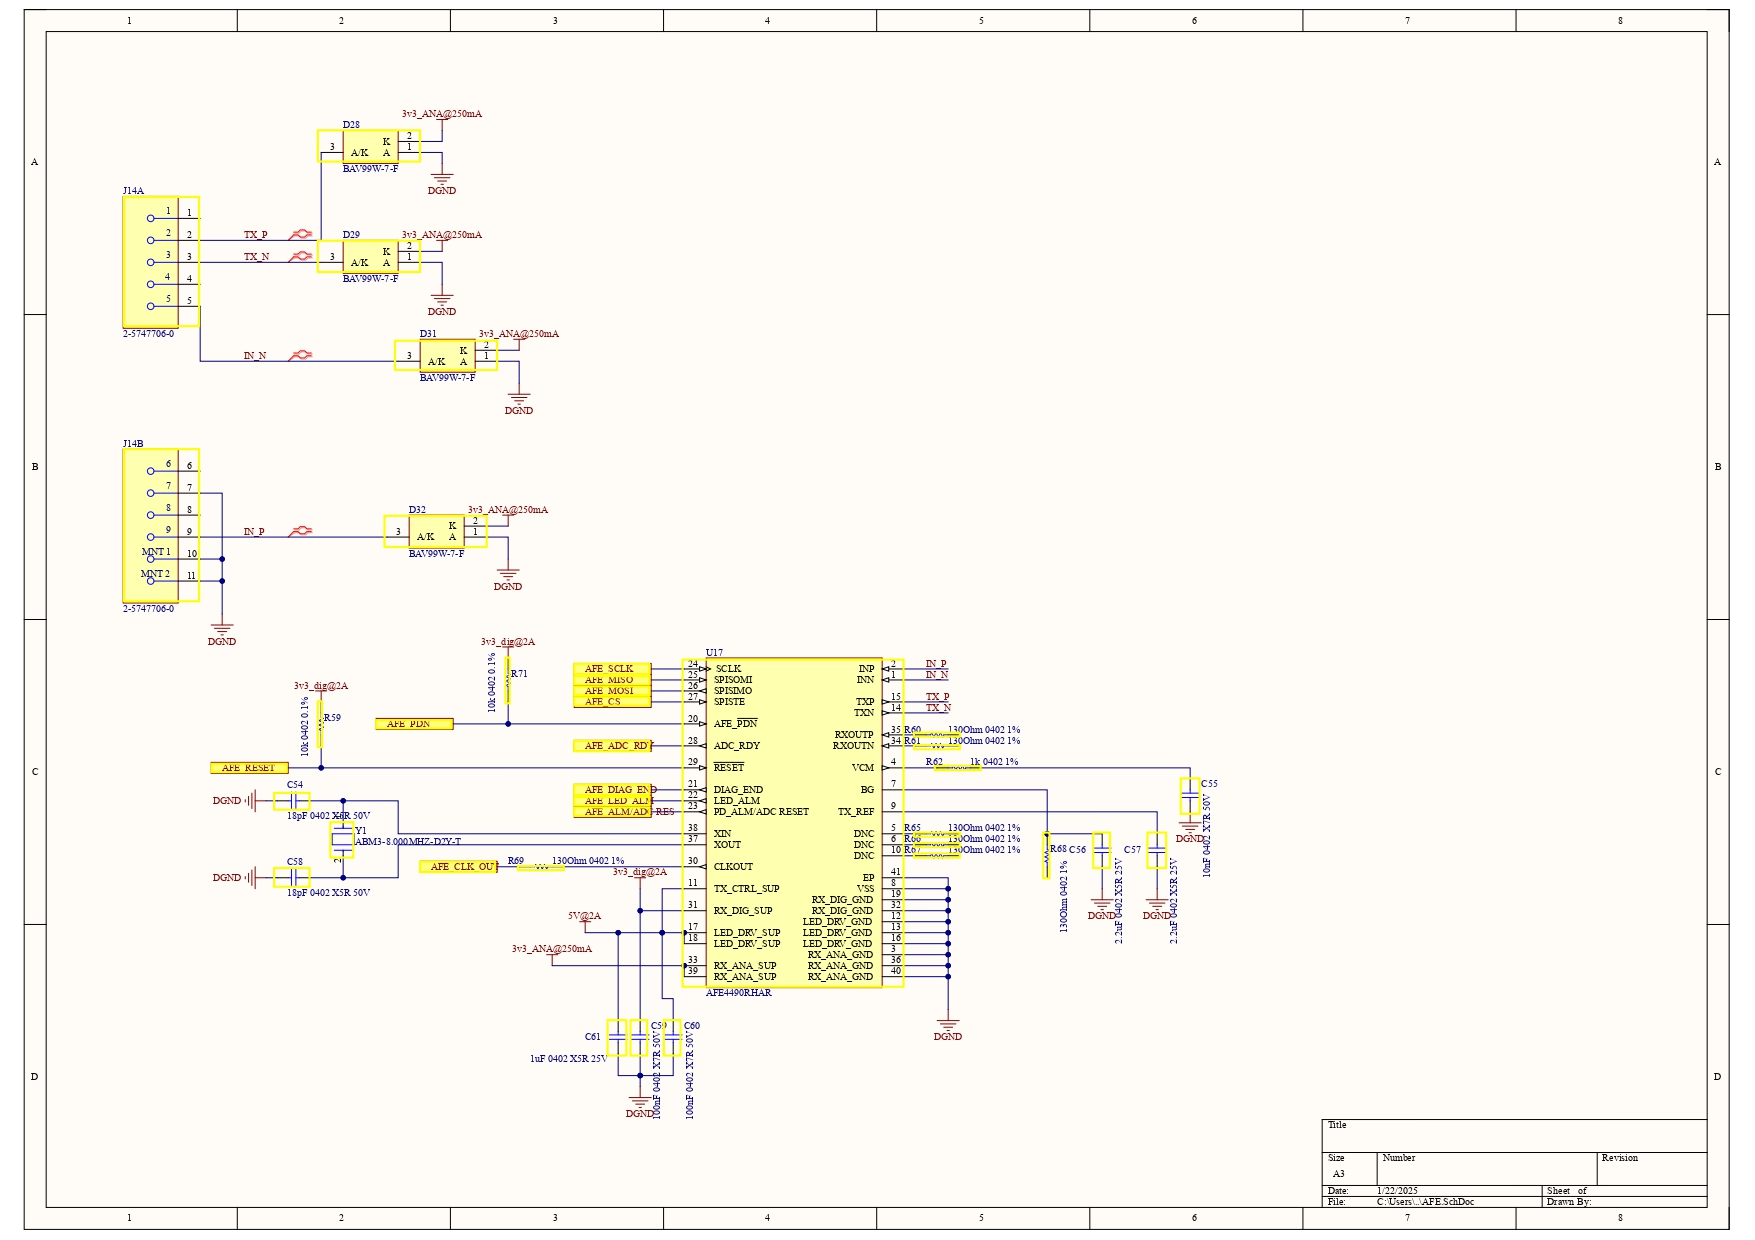
\includegraphics[width=1\textwidth]{img/AFE.jpg}
\caption{Esquema eléctrico del circuito AFE4490, incluyendo alimentación analógica y digital, señales de control y líneas SPI de comunicación con el microcontrolador. Extraído del fichero \texttt{AFE.SchDoc}. Fuente: \href{https://medicalopenworld.org/}{MedicalOpenWorld}.}
\end{figure}

Físicamente, en el hardware, el AFE4490 se encuentra en el reverso de la PCB, es de muy pequeño tamaño y tiene este aspecto:

\begin{figure}[H]
    \centering
    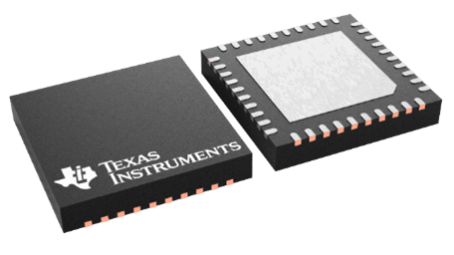
\includegraphics[width=0.5\linewidth]{img/AFE.png}
    \caption{Extremo frontal analógico integrado (AFE) para pulsioxímetros. Imagen referencial del componente físico AFE4490. Fuente: \href{https://www.ti.com/product/es-mx/AFE4490/part-details/AFE4490RHAT}{TexasInstruments.}}
    \label{fig:AFE2}
\end{figure}


\subsection{Gestión de alimentación y carga de batería}

Este plano muestra la parte del circuito que permite alimentar todo el sistema a partir de una batería de 12V. Es importante fijarse en los reguladores de tensión que convierten esa entrada a los 3.3V necesarios para el AFE4490 y el ESP32. 


\begin{figure}[H]
    \centering
    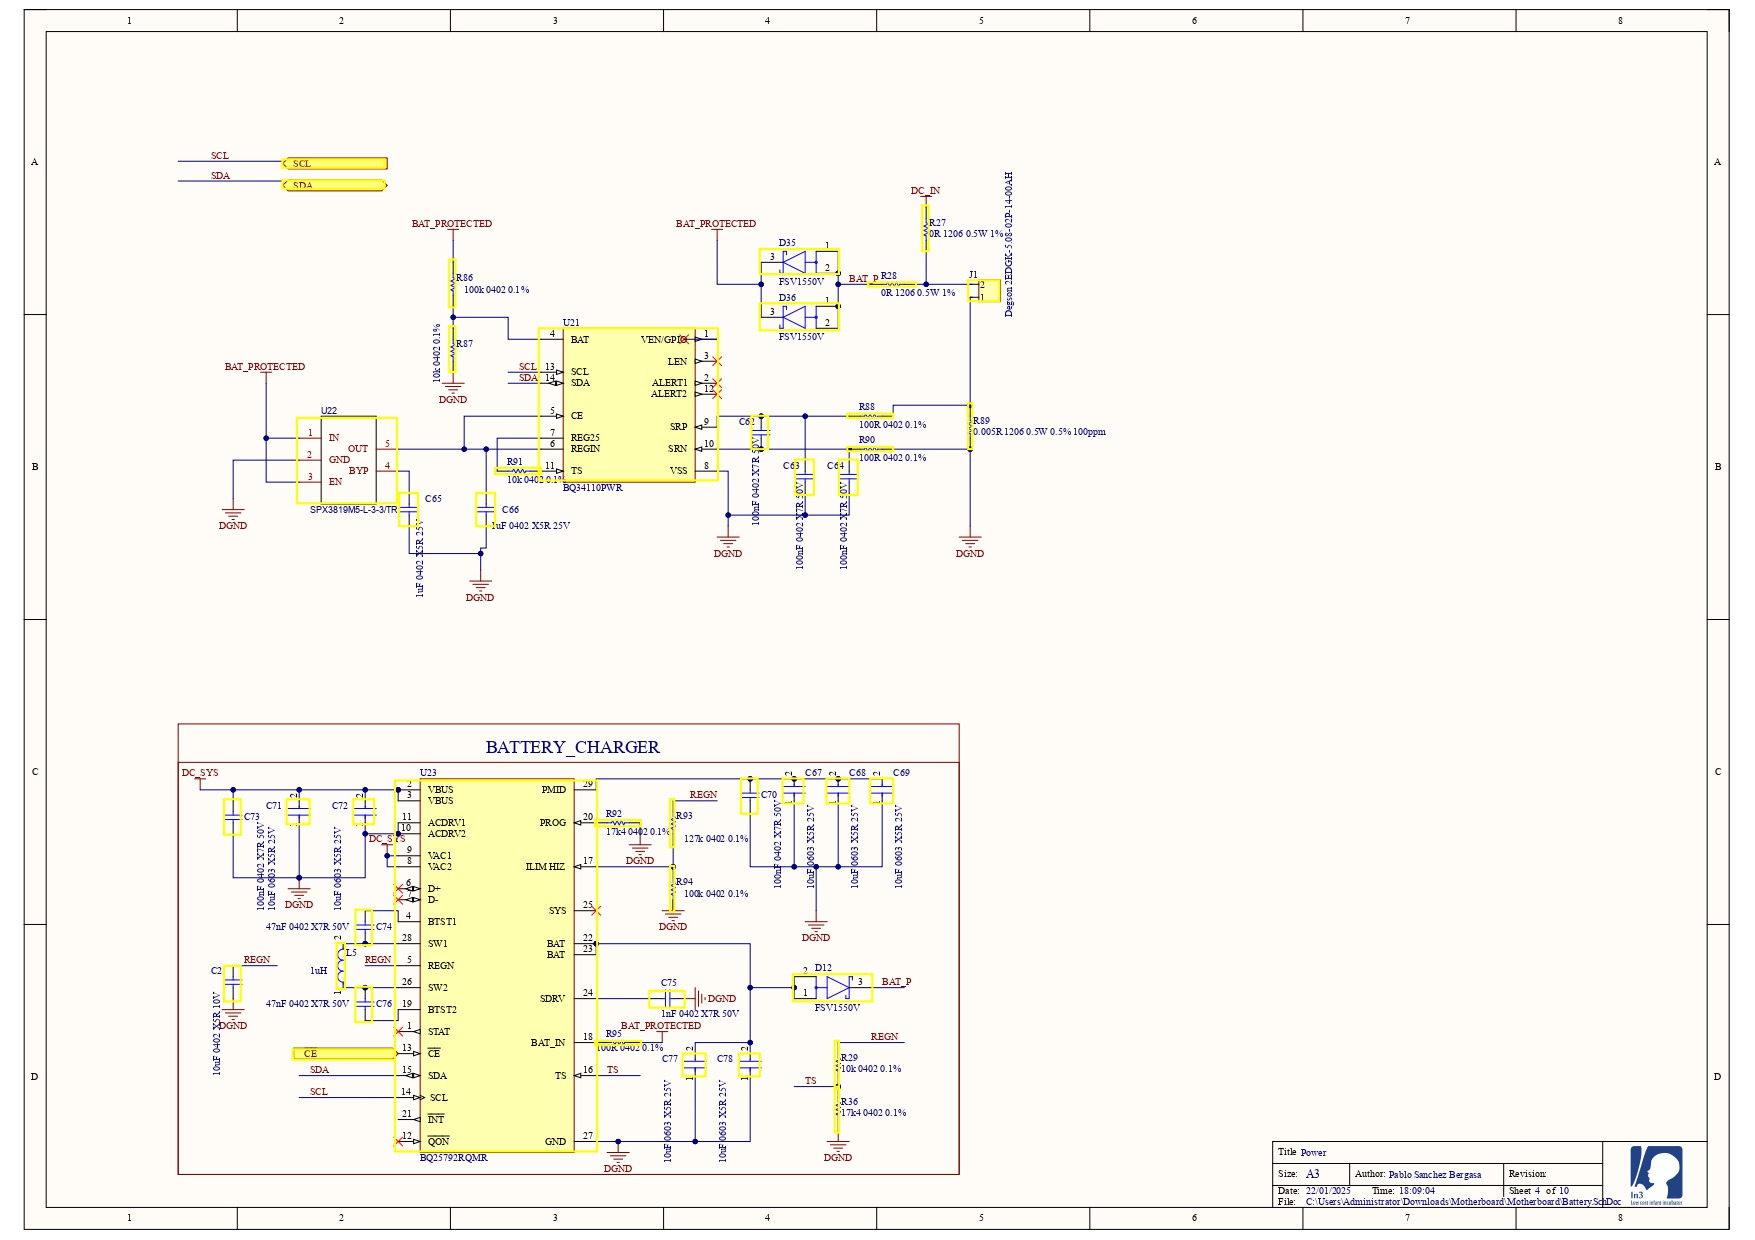
\includegraphics[width=1\linewidth]{img/Battery.jpg}
    \caption{Esquema de alimentación del sistema, donde se aprecia la fuente principal de 5V, la conversión a 3.3V digital y analógico, y la distribución de potencia hacia el AFE y el microcontrolador. Extraído del fichero \texttt{Power\_Input.SchDoc}. Fuente: \href{https://medicalopenworld.org/}{MedicalOpenWorld}}
    \label{fig:Battery}
\end{figure}

\subsection{Microcontrolador ESP32}

Este es el cerebro del sistema. En el plano se puede localizar el microcontrolador ESP32-WROOM-32, sus pines de entrada/salida y las conexiones hacia el AFE4490 mediante el bus SPI. Lo importante es fijarse en la relación entre los pines marcados como MOSI, MISO, SCK y CS, y las señales que se intercambian con el AFE.


\begin{figure}[H]
\centering
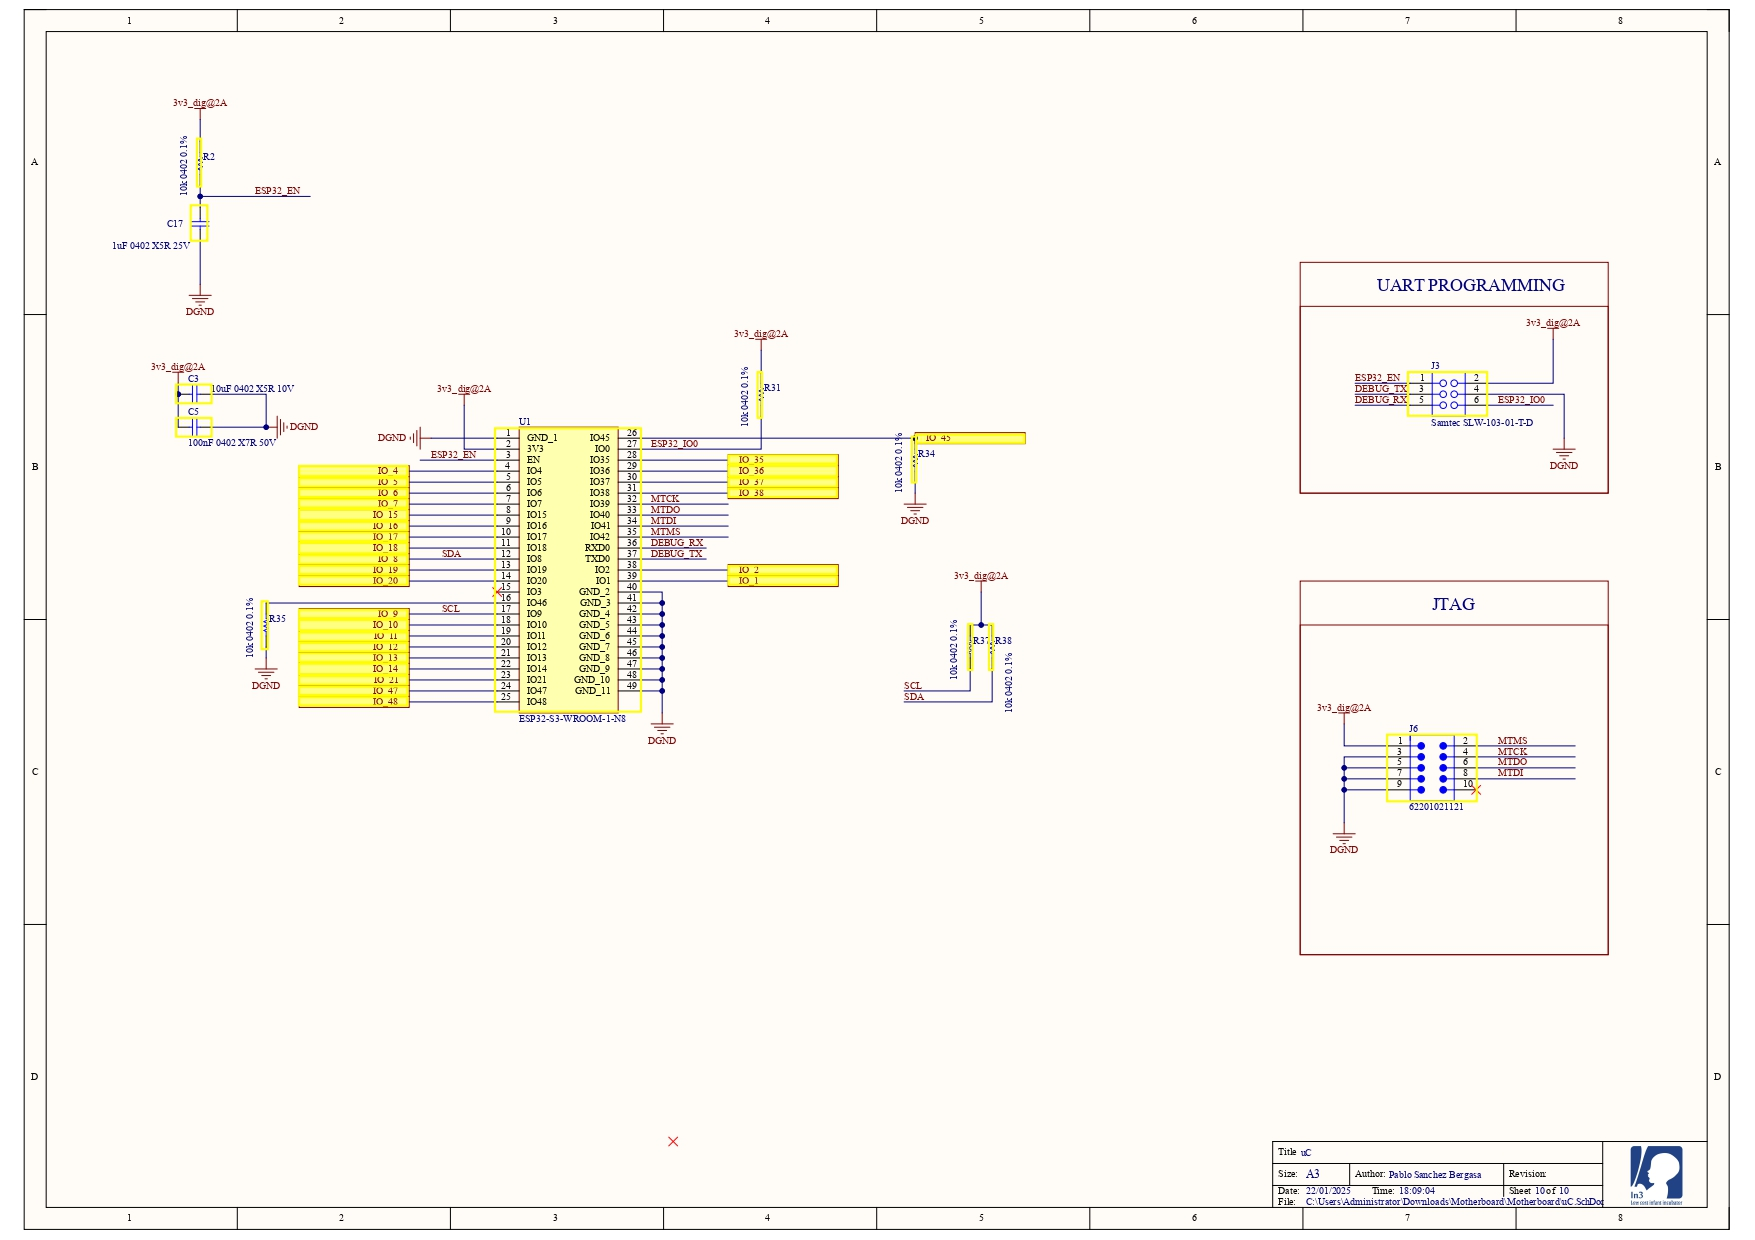
\includegraphics[width=1\textwidth]{img/Uc.jpg}
\caption{Plano del microcontrolador ESP32-WROOM-32. Extraído del fichero \texttt{Uc.SchDoc} Fuente: \href{https://medicalopenworld.org/}{MedicalOpenWorld} }
\end{figure}


Estos esquemas permitieron visualizar al inicio del proyecto cómo se integran a nivel de hardware los principales componentes implicados en la adquisición de señales PPG, así como su conexión con el microcontrolador que ejecuta el firmware desarrollado. 


\section{Diseño arquitectónico}

Dado que este proyecto no corresponde a una aplicación móvil o de escritorio, basada en objetos, sino a un sistema embebido de adquisición y procesamiento de señales biomédicas, se ha optado por no incluir diagramas clásicos como los de clases, secuencia o despliegue.

En su lugar, esta sección incluye diagramas de bloques que describen el comportamiento de los algoritmos implementados para la estimación de frecuencia cardíaca y SpO$_2$, basados en las señales adquiridas por el sensor. Estos diagramas reflejan las etapas de procesamiento y el flujo de datos desde la adquisición hasta el cálculo final de los parámetros fisiológicos.

\subsection{Algoritmos de estimación de la frecuencia cardíaca}

Los algoritmos que se muestran a continuación se han aplicado sobre los archivos CSV generados a partir del sistema de adquisición de datos descrito en el Anexo D y en la metodología de la memoria.

A continuación, se presentan los diagramas de los dos métodos que ofrecieron mejores resultados para la estimación de la frecuencia cardíaca, basados ambos en la detección de picos de la señal PPG, pero con enfoques distintos de preprocesamiento.

\subsubsection{Algoritmo 1: Filtro de media móvil}

El código correspondiente a este algoritmo se encuentra en el notebook \texttt{spo2.ipynb}. Los pasos seguidos se representan en la figura \ref{fig: diagrama1}.

\begin{figure}[H]
    \centering
    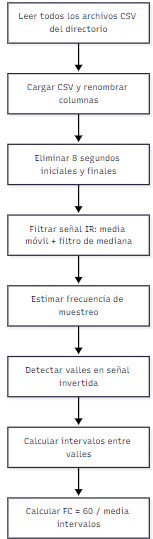
\includegraphics[scale = 0.65]{img/medias_moviles.png}
    \caption{Diagrama de bloques del algoritmo de frecuencia cardíaca basado en media móvil. \textit{Elaboración propia.}}
    \label{fig: diagrama1}
\end{figure}

\subsubsection{Algoritmo 2: Filtro paso bajo y detección con SciPy}

El código correspondiente a este algoritmo se encuentra en el notebook \texttt{pulsi\_comercial.ipynb}.El proceso se muestra en la figura \ref{fig: paso_bajo2}.

\begin{figure}[H]
    \centering
    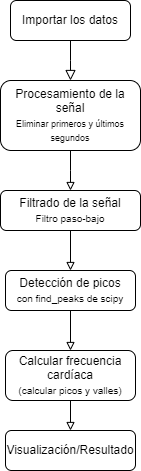
\includegraphics[scale = 0.65]{img/paso_bajo.png}
    \caption{Diagrama de bloques del algoritmo de frecuencia cardíaca con filtrado paso-bajo y detección por picos.\textit{Elaboración propia.}}
    \label{fig: paso_bajo2}
\end{figure}

Como se defendió en la metodología de la memoria teórica, se escogió el método que utiliza el preprocesamiento con media móvil + mediana. La elección entre uno u otro dependió del nivel de optimización y el coste computacional.

\subsection{Algoritmos de estimación de la saturación de oxígeno}

Para el cálculo de la SpO$_2$, inicialmente se desarrollaron versiones sencillas que aplicaban el cálculo clásico del ratio con aproximaciones teóricas o coeficientes fijos. Sin embargo, los mejores resultados se obtuvieron con los siguientes enfoques:

\subsubsection{Algoritmo 1: método de Ratio of Ratios y fórmula cuadrática }

El código correspondiente a este algoritmo se encuentra en el notebook \texttt{spO2\_algo\_v4.ipynb}.El proceso se muestra en la figura \ref{fig: SpO2_algo_v4}.

\begin{figure}[H]
    \centering
    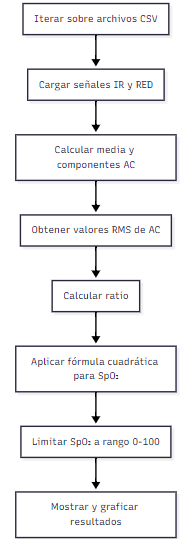
\includegraphics[width=0.25\linewidth]{img/SpO2_algo_v4.png}
    \caption{Diagrama de bloques del algoritmo de estimación de SpO$_2$ por Ratio y fórmula cuadrática. \textit{Elaboración propia.}}
    \label{fig: SpO2_algo_v4}
\end{figure}

\subsubsection{Algoritmo 2: mediante ratio AC/DC y modelo lineal calibrado}

El desarrollo de este algoritmo está implementado en el notebook \texttt{tabla\_LUT.ipynb}, cuyo funcionamiento se ilustra en la figura~\ref{fig:tabla_LUT2}.


\begin{figure}[H]
    \centering
    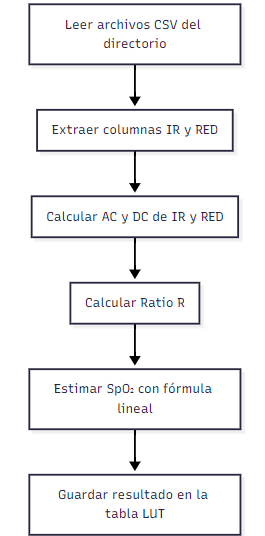
\includegraphics[width=0.25\linewidth]{img/tabla_LUT.png}
    \caption{Diagrama de bloques del algoritmo de estimación de SpO$_2$ por Ratio y modelo lineal. \textit{Elaboración propia.}}
    \label{fig:tabla_LUT2}
\end{figure}


\subsubsection{Algoritmo 3: Estimación por regresión lineal}

El algoritmo descrito puede consultarse en el notebook \texttt{Paper\_CS.ipynb}. Su flujo de ejecución se representa en la figura~\ref{fig: Paper_CS2}.

\begin{figure}[H]
    \centering
    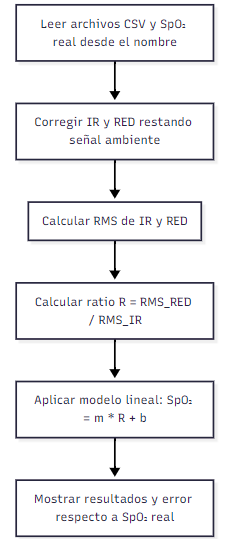
\includegraphics[scale=0.5]{img/Paper_CS.png}
    \caption{Diagrama de bloques del algoritmo de estimación de SpO$_2$ por regresión lineal.\textit{Elaboración propia.}}
    \label{fig: Paper_CS2}
\end{figure}

\subsubsection{Algoritmo 4: Estimación mediante tabla personalizada}

La implementación detallada de este algoritmo se encuentra en el notebook \texttt{uch\_spo2\_table.ipynb}. La figura~\ref{fig: uch_spo2_table2} muestra de forma esquemática su estructura y funcionamiento.

\begin{figure}[H]
    \centering
    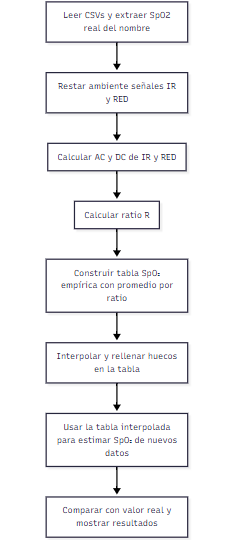
\includegraphics[scale =0.6]{img/uch_spo2_table.png}
    \caption{Diagrama de bloques del algoritmo de estimación de SpO$_2$ basado en tabla personalizada.\textit{Elaboración propia.}}
    \label{fig: uch_spo2_table2}
\end{figure}

\newpage

\subsection{Algoritmo final en el firmware}


\begin{figure}[H]
    \centering
    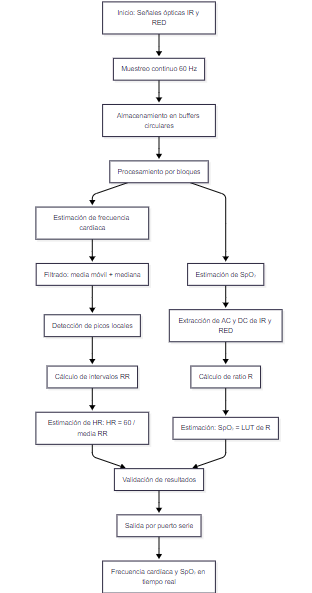
\includegraphics[width=0.75\linewidth]{img/flujo_firmware.png}
    \caption{Algoritmo de estimación de ambos parámetros en el propio firmware. El algoritmo ha sido explicado en la sección de metodología de la memoria.\textit{Elaboración propia.}}
    \label{fig:flujo_firmware}
\end{figure}
\apendice{Especificación de Requisitos}

Este anexo ha sido adaptado con la información que define el desarrollo realizado, ya que, aunque no se trata de un sistema con interacción directa con el usuario, la solución propuesta incluye funcionalidades software.


En este proyecto existe una lógica funcional bien definida, estructurada en tareas del firmware, que interactúa tanto con los sensores físicos como con el usuario investigador a través del puerto serie. Por ello, se ha definido un caso de uso técnico que representa el comportamiento del sistema en relación con la adquisición, procesamiento y extracción de datos biomédicos.

\section{Diagrama de casos de uso}

\begin{figure}[H]
    \centering
    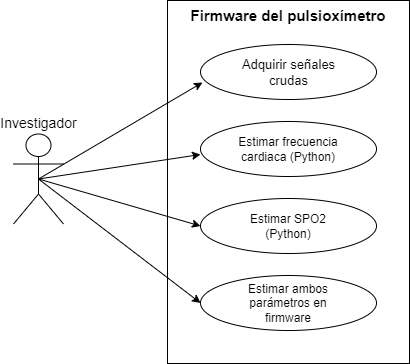
\includegraphics[scale =0.43]{img/casodeuso1.png}
    \caption{CU-1. \textit{Elaboración propia}}
    \label{fig:casos_uso}
\end{figure}



\section{Explicación casos de uso.}

\begin{table}[H]
	\centering
	\begin{tabularx}{\linewidth}{ p{0.21\columnwidth} p{0.71\columnwidth} }
		\toprule
		\textbf{CU-1}    & \textbf{Adquirir señales crudas} \\
		\toprule
		\textbf{Versión}              & 1.0 \\
		\textbf{Autor}                & Elena Ruiz \\
		\textbf{Descripción}          & El sistema adquiere señales fotopletismográficas crudas del sensor U401-D a través del AFE4490 y las envía al PC mediante comunicación serie. Los datos son almacenados en formato csv para su posterior análisis.\\
		\textbf{Precondición}         & El sensor debe estar correctamente conectado y alimentado. El microcontrolador debe haber iniciado correctamente el firmware. \\
		\textbf{Acciones}             &
		\begin{enumerate}
			\item Conectar los elementos necesarios del sistema hardware.
			\item Asegurar la correcta conexión y el reconocimiento de la placa por el ordenador.
			\item Registrar un log individual a la vez que se están midiendo los valores con un pulsioximetro externo de referencia.
			\item Guardar los datos en un archivo CSV mediante un script en Python.
		\end{enumerate} \\
		\textbf{Postcondición}        & Se genera un archivo CSV con las señales crudas. \\
		\textbf{Excepciones}          & Pérdida de comunicación serie, fallo en la alimentación del sensor, datos corruptos. \\
		\textbf{Importancia}          & Alta \\
		\bottomrule
	\end{tabularx}
	\caption{CU-1 Adquirir señales crudas. \textit{Elaboración propia.}}
\end{table}


\begin{table}[H]
	\centering
	\begin{tabularx}{\linewidth}{ p{0.21\columnwidth} p{0.71\columnwidth} }
		\toprule
		\textbf{CU-2}    & \textbf{Estimar frecuencia cardiaca (Python)} \\
		\toprule
		\textbf{Versión}              & 1.0 \\
		\textbf{Autor}                & Elena Ruiz \\
		\textbf{Descripción}          & El sistema procesa la señal PPG en formato .csv para detectar picos y calcular la frecuencia cardíaca en tiempo no real utilizando scripts en Python. \\
		\textbf{Precondición}         & El archivo CSV con datos crudos debe existir y estar completo. \\
		\textbf{Acciones}             &
		\begin{enumerate}
			\item Cargar el archivo CSV con las señales IR y/o RED.
			\item Aplicar filtrado.
			\item Detectar picos correspondientes a los latidos.
			\item Calcular la frecuencia cardíaca media (en BPM).
		\end{enumerate} \\
		\textbf{Postcondición}        & Se obtiene un valor estimado de frecuencia cardíaca, que puede compararse con la referencia externa. Los algoritmos que mejor resultados ofrecen son estudiados posteriormente para ser implementados en el firmware.\\
		\textbf{Excepciones}          & Señal demasiado ruidosa, número insuficiente de picos, error de formato en CSV. \\
		\textbf{Importancia}          & Alta \\
		\bottomrule
	\end{tabularx}
	\caption{CU-2 Estimar frecuencia cardiaca (Python). \textit{Elaboración propia.}}
\end{table}

\begin{table}[H]
	\centering
	\begin{tabularx}{\linewidth}{ p{0.21\columnwidth} p{0.71\columnwidth} }
		\toprule
		\textbf{CU-3}    & \textbf{Estimar SpO$_2$ (Python)} \\
		\toprule
		\textbf{Versión}              & 1.0 \\
		\textbf{Autor}                & Elena Ruiz \\
		\textbf{Descripción}          & El sistema calcula la saturación de oxígeno estimada a partir del cociente de las señales PPG. \\
		\textbf{Precondición}         & El archivo CSV debe contener las señales correctamente sincronizadas y calibradas. \\
		\textbf{Acciones}             &
		\begin{enumerate}
			\item Cargar y recortar las señales.
			\item Aplicar filtros a las señales RED e IR.
			\item Calcular componentes AC y DC mediante media y picos.
			\item Obtener el índice R = (ACred/DCred) / (ACir/DCir).
			\item Estimar SpO$_2$ con tabla LUT o regresión calibrada.
		\end{enumerate} \\
		\textbf{Postcondición}        & Se muestra el valor estimado de SpO$_2$ para la sesión analizada. \\
		\textbf{Excepciones}          & Cálculo inválido por baja perfusión, señales ruidosas o relación R fuera del rango. Los algoritmos que mejor resultados ofrecen son estudiados posteriormente para ser implementados en el firmware. \\
		\textbf{Importancia}          & Alta \\
		\bottomrule
	\end{tabularx}
	\caption{CU-3 Estimar SpO$_2$ (Python). \textit{Elaboración propia.}}
\end{table}

\begin{table}[H]
	\centering
	\begin{tabularx}{\linewidth}{ p{0.21\columnwidth} p{0.71\columnwidth} }
		\toprule
		\textbf{CU-4}    & \textbf{Estimar frecuencia cardíaca y SpO$_2$ (firmware)} \\
		\toprule
		\textbf{Versión}              & 1.0 \\
		\textbf{Autor}                & Elena Ruiz \\
		\textbf{Descripción}          & El firmware del microcontrolador procesa las señales PPG en tiempo real para calcular la frecuencia cardíaca y la saturación de oxígeno utilizando los algoritmos previamente probados en entorno Python. \\
		\textbf{Precondición}         & Sensor y AFE correctamente inicializados, condiciones de señal adecuadas, adquisición continua activada. \\
		\textbf{Acciones}             &
		\begin{enumerate}
			\item Leer muestras IR y RED desde el AFE4490.
			\item Aplicar los algoritmos estudiados que han sido implementados en C++.
			\item Mostrar Frecuencia cardiaca y SpO$_2$ por UART al PC.
            \item Comparar resultado en tiempo real con un pulsioxímetro externo de referencia.
		\end{enumerate} \\
		\textbf{Postcondición}        & Se envían los valores estimados de HR y SpO$_2$ al sistema de monitorización y/o se muestran en pantalla. \\
		\textbf{Excepciones}          & Datos erróneos por movimiento, baja señal o demasiada intensidad de luz.\\
		\textbf{Importancia}          & Muy alta \\
		\bottomrule
	\end{tabularx}
	\caption{CU-4 Estimar frecuencia cardíaca y SpO$_2$ (firmware). \textit{Elaboración propia.}}
\end{table}


\section{Prototipos de interfaz o interacción con el proyecto.}

El sistema implementado, en el grado de desarrollo en el que se encuentra, no dispone de una interfaz gráfica de usuario avanzada. Sin embargo, se han considerado dos formas de interacción o visualización con el sistema:

\subsection{Salida por terminal serie}

Durante el desarrollo y las pruebas del sistema, la información de frecuencia cardíaca y saturación de oxígeno estimada en firmware se muestra por consola a través del puerto serie, utilizando el monitor serial de Visual Studio Code. En la Figura \ref{fig: Captura_firmware} puede observarse una captura de la salida real del sistema, donde se visualizan los valores estimados por el microcontrolador en tiempo real.

\begin{figure}[H]
    \centering
    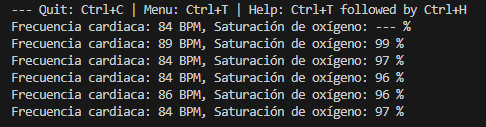
\includegraphics[width=0.7\textwidth]{img/Captura_firmware.png}
    \caption{Salida de datos del pulsioxímetro por consola serie (Visual Studio Code). \textit{Elaboración propia.}}
    \label{fig: Captura_firmware}
\end{figure}

\subsection{Interfaz en pantalla integrada (prototipo simulado)}

Idealmente, los valores deberían visualizarse en el display integrado en la incubadora neonatal (pantalla TFT). Sin embargo, por limitaciones técnicas y de tiempo, esta parte no ha podido completarse durante el desarrollo del TFG. Para reflejar la intención de diseño, se ha generado un prototipo gráfico (Figura \ref{fig:display_mockup}) que representa cómo se espera mostrar la información final en el dispositivo. En dicha interfaz se muestran los valores de temperatura, humedad, SpO$_2$ y frecuencia cardíaca en un formato claro, accesible y compatible con el resto de la interfaz de la incubadora.

\begin{figure}[H]
    \centering
    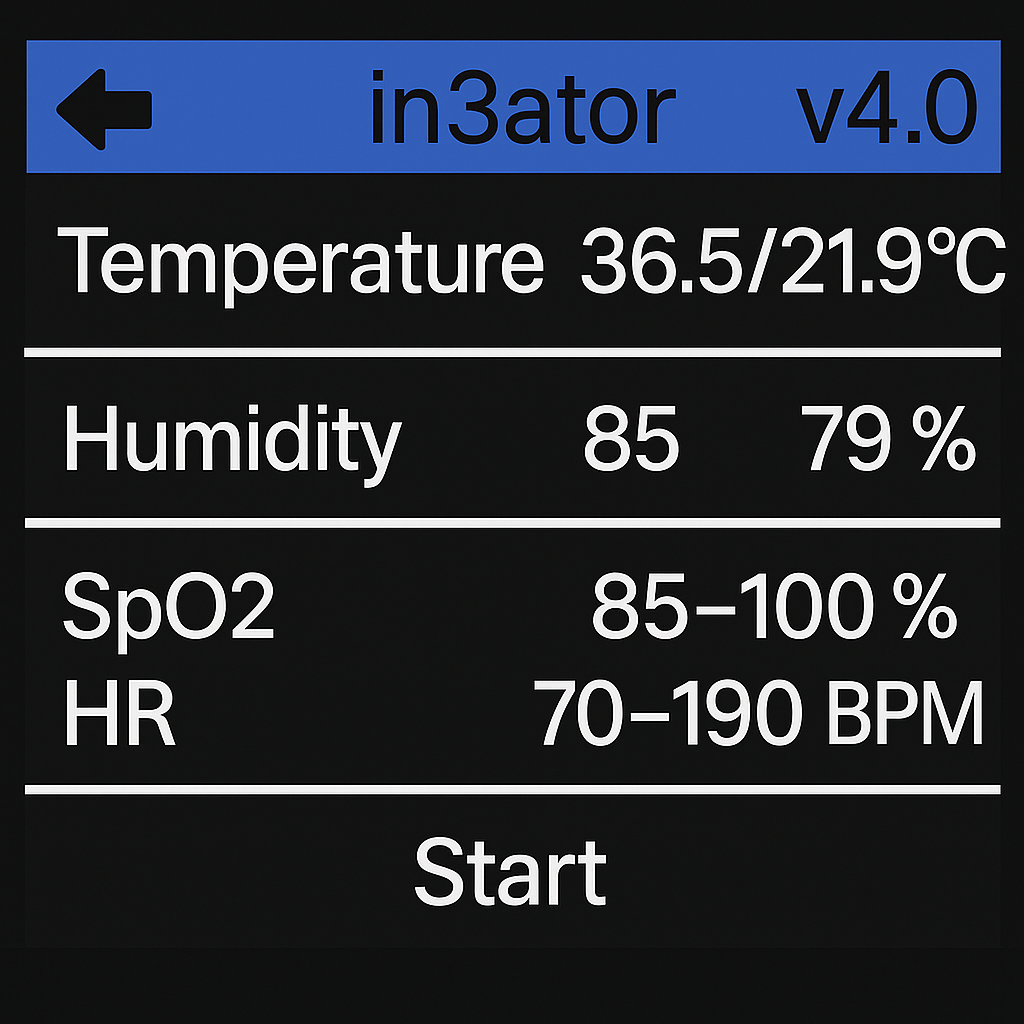
\includegraphics[width=0.3\textwidth]{img/display.png}
    \caption{Prototipo simulado de la interfaz final en el display de la incubadora. \textit{Elaboración propia.}}
    \label{fig:display_mockup}
\end{figure}







\apendice{Estudio experimental}

Este anexo recoge de forma detallada el trabajo experimental desarrollado a lo largo del proyecto, incluyendo tanto las fases de diseño, configuración e implementación como los procesos iterativos de prueba, validación y corrección. Se documentan los pasos seguidos para la adquisición y procesamiento de señales del pulsioxímetro integrado en la incubadora \textit{In$^3$ator}, con especial énfasis en los resultados erróneos o no válidos obtenidos durante el desarrollo, y en el análisis técnico realizado hasta alcanzar resultados fiables y representativos.

\section{Cuaderno de trabajo.}

\subsection{Fase de análisis e integración del sistema }

Para comenzar con el proyecto, disponíamos de material ya desarrollado por el equipo \textit{In$^3$ator}, por lo que comenzamos con una fase de análisis del sistema de la incubadora. Se estudió el sensor óptico UA401-D, el AFE4490 como front-end analógico, y los esquemas eléctricos de la PCB. También fue necesario familiarizarse con el entorno de desarrollo PlatformIO y con el código existente, el cual presentaba una estructura poco modular y escasamente documentada. Estas limitaciones iniciales dificultaron la acción directa sobre el código y marcaron el comienzo de una fase de rediseño centrada en la adquisición de datos crudos. 

La importación del proyecto al entorno de desarrollo resultó algo compleja, ya que al tratarse de un sistema completo para el funcionamiento de toda la incubadora (no solo del módulo de pulsioximetría), contenía una gran cantidad de líneas de código, clases, librerías y dependencias, lo que dificultaba su carga y ralentizaba el sistema. 
Además, el firmware no podía exportarse ni compilarse desde cualquier ruta del sistema de archivos, lo que obligó a reorganizar manualmente los directorios y ajustar varias configuraciones de PlatformIO para poder compilarlo correctamente. 

Igualmente, fue necesario realizar tareas de hardware que no estaban previstas, como la soldadura de algunos pines en la PCB para permitir la conexión con el programador. No disponía del material ni de los conocimientos necesarios para realizar esta tarea por mi cuenta, por lo que fue imprescindible acudir al laboratorio, donde el tutor me ayudó a realizar correctamente la soldadura.  Esta tarea permitió establecer la comunicación entre el microcontrolador y el programador, para que el ordenador pudiera leer los datos que se querían registrar.

Superada esta etapa, surgieron nuevas dificultades relacionadas con el cableado. El cable proporcionado inicialmente era de tipo USB-C, incompatible con el programador utilizado, que requería una conexión microUSB. Una vez conseguido el cable adecuado, persistieron los errores de comunicación: el ordenador no reconocía el dispositivo porque el conector no hacía buen contacto físico con la clavija del programador. Tras varias comprobaciones, se logró estabilizar la conexión aplicando presión manual para ajustar mejor el cable al puerto. Fue entonces cuando, finalmente, se consiguió visualizar por pantalla los datos crudos del sensor en tiempo real, lo que permitió, por primera vez, dar inicio a la fase de adquisición y análisis de señales. 

\subsection{Adquisición de datos y análisis preliminar de señales}

Una vez conseguida la visualización en tiempo real de los datos crudos del sensor a través del puerto serie, el siguiente paso fue intentar adaptar el código del firmware para estructurar los datos en un formato más manejable. El código base ya generaba continuamente las cuatro señales que proporciona el AFE4490 (\texttt{IR}, \texttt{AMB\_IR}, \texttt{RED}, \texttt{AMB\_RED}), pero debido a la complejidad del firmware y a la falta de experiencia previa en su estructura, resultaba difícil intervenir directamente sobre él. Por ello, se optó por avanzar en paralelo capturando los datos en formato \texttt{.csv} y realizar el procesamiento y análisis por separado en un entorno controlado como Python, que es lo que principalmente se ha utilizado en la carrera. 

No obstante, para poder adaptar correctamente el flujo de adquisición, fue necesario modificar la función \texttt{get\_AFE44XX\_Data()} del archivo fuente \texttt{spo2.cpp}, con el fin de tener una referencia temporal en milisegundos e imprimir las señales por el puerto serie de forma estructurada. También se añadió una condición para limitar la duración de cada registro a 30 segundos y se introdujo un control de tiempo basado en \texttt{delayMicroseconds()} para mantener una frecuencia de adquisición cercana a 60~Hz, adecuada para el posterior análisis.

En paralelo, se desarrollaron dos versiones del script en Python para capturar y almacenar los datos del sensor. La primera versión, \texttt{save\_log.py}, permitió comprobar la recepción de datos en el equipo, pero presentaba varias limitaciones que fueron señaladas durante una revisión con el tutor: la frecuencia de muestreo era demasiado baja, solo se registraban dos señales (en lugar de las cuatro disponibles, esto debido a un error en la modificación de la función) y no se incluía una cabecera descriptiva en el archivo.

A raíz de estos comentarios, se desarrolló una segunda versión mejorada, tanto del firmware como del script. En el caso de la función principal \texttt{get\_AFE44XX\_Data()}, se aplicaron los ajustes mencionados para la temporización, la duración de captura y la salida de datos completa por el puerto serie. En cuanto al nuevo script \texttt{save\_log2.py}, se programó para recibir correctamente las cinco variables por el puerto serie (incluido el tiempo en ms), incluir una cabecera con los nombres de las columnas, mostrar los datos en tiempo real por consola, y guardar automáticamente cada sesión en un archivo \texttt{.csv}. Además, se nombró cada archivo en el formato \texttt{raw\_data\_SpO2\_HR.csv}, incluyendo en él los valores de SpO\textsubscript{2} y frecuencia cardíaca obtenidos manualmente al final de cada registro con dispositivos comerciales colocados en la mano contraria.


Durante esta fase se realizaron numerosas sesiones de adquisición, todas ellas de 30 segundos. En los primeros registros comenzaron a aparecer algunos problemas técnicos. En ocasiones, las señales presentaban interferencias por ruido o artefactos por movimiento e incluso había registros con los que se obtenían valores constantes, seguramente por la mala colocación del dedo o por la presencia de demasiada luz. Además, en situaciones en las que se intentaba aumentar el ritmo cardíaco (saltando o subiendo escaleras), aparecían crecimientos prolongados en la forma de onda que dificultaban el cálculo de la línea base, provocando errores en los algoritmos de análisis. Estos registros se conservaron inicialmente para su estudio posterior, aunque algunos fueron eliminados por considerarse no utilizables.

A lo largo de esta etapa se generaron aproximadamente entre 30 y 40 registros. La clasificación en señales válidas o no válidas no se realizó en un primer momento, sino que fue introducida más adelante como parte del proceso de validación de los algoritmos. En un primer análisis visual mediante notebooks en Jupyter, se detectaron señales inestables o con valores fuera de rango. Por ello, se hizo una primera eliminación basada en inspección visual, complementada más tarde por la validación de los parámetros calculados, descartando aquellos que presentaban valores fisiológicamente imposibles.

También se decidió, en una fase posterior, recortar el inicio y el final de cada registro para eliminar los efectos transitorios asociados a la colocación del sensor. Inicialmente se planteó eliminar de forma general los primeros y últimos 5 segundos, pero con el tiempo se optó por realizar un recorte personalizado para cada señal, analizando de forma manual qué segmentos eran realmente válidos en cada caso.

\subsection{Procesamiento de señales}
En el momento en el que se registraron suficientes señales como para realizar un análisis que permitiera comparar resultados, se procedió a la estimación de los dos principales parámetros que queríamos obtener del pulsioxímetro: la frecuencia cardíaca y la saturación de oxígeno en sangre. Inicialmente, se intentó calcular ambos valores al mismo tiempo, pero más tarde decidimos tratar de sacar ambos procedimientos por separado, al ver que iba a ser más complicado de lo esperado. Se comenzó con el cálculo de la frecuencia cardíaca al tratarse de un método menos costoso y más fácil de entender.

Antes de obtener resultados válidos, se probaron varios métodos de procesamiento de señal que no ofrecieron resultados satisfactorios. Estos ensayos fueron necesarios para explorar diferentes enfoques, pero en muchos casos los resultados obtenidos fueron erróneos o imposibles.

Uno de los primeros métodos consistió en aplicar filtros paso bajo simples directamente sobre la señal IR, sin realizar ninguna corrección por luz ambiente. Aunque la señal se suavizaba visualmente, no era suficiente para eliminar el ruido, y los picos resultaban confusos o poco definidos. En algunos casos, el filtrado excesivo eliminaba también la componente pulsátil de interés, provocando señales distorsionadas.

Se descubrió que modificando los parámetros de los filtros empleados, se mejoraba la estimación, sin embargo, estos cambios no servían para todos los registros y, además no seguían ningún patrón que pudiera servir de ayuda para obtener mejores resultados, si no que era puro azar.

En otros intentos se aplicó directamente la detección de picos sin un preprocesamiento adecuado. Esto provocó resultados fuera del rango fisiológico, debido a la sensibilidad del algoritmo a pequeñas variaciones del ruido. En algunos casos no se detectaban picos, y en otros se detectaban muchos falsos positivos, lo que impedía obtener estimaciones fiables.

También se realizaron pruebas comparando directamente las señales IR y RED sin aplicar filtros ni correcciones. Estas señales presentaban un nivel de ruido elevado y estructuras poco claras, lo que dificultaba cualquier análisis cuantitativo.

Por último, se intentó adaptar algoritmos externos desarrollados para otros sensores o condiciones distintas, pero sus escalas, unidades o características de adquisición no eran compatibles con los datos reales obtenidos, por lo que no ofrecieron ningún resultado útil.

Aunque todos estos métodos fallaron, permitieron identificar errores comunes como la ausencia de corrección de luz ambiente, la necesidad de un mejor filtrado, y la importancia de ajustar correctamente los parámetros del algoritmo de detección.  Uno de los mayores errores iniciales fue no recortar los tramos de señal con interferencias (especialmente al inicio y final del registro), por temor a perder información útil. Sin embargo, se comprobó posteriormente que mantener estos segmentos comprometía gravemente la calidad del análisis. 

Tras los primeros intentos fallidos, se definieron y aplicaron una serie de métodos que ofrecieron resultados razonables y estables, tanto para la estimación de la frecuencia cardíaca como de la saturación de oxígeno. Estos métodos se diseñaron teniendo en cuenta las limitaciones observadas previamente y con un enfoque progresivo, basado en pruebas controladas.

Para el cálculo de la frecuencia cardíaca, el enfoque más efectivo consistió en aplicar un filtrado suave a la señal IR corregida por luz ambiente. Los métodos que ofrecieron mejores resultados fueron la media móvil junto con el filtro de mediana y el filtro paso-bajo Butterworth, que permitían reducir el ruido sin deformar la componente pulsátil. A diferencia de los primeros intentos, en este caso se ajustaron los parámetros de la ventana de filtrado y se aplicó sobre señales ya recortadas, eliminando los tramos iniciales y finales donde se acumulaban artefactos (personalizados para cada señal).

Una vez filtrada la señal, se utilizó un algoritmo de detección de picos que incorporaba una distancia mínima entre pulsos. La configuración de estos parámetros permitió eliminar falsos positivos y garantizar que cada pico detectado correspondiera a un latido. En la mayoría de los casos, se utilizó la señal IR, ya que se comprobó que era más estable que la señal RED.

Con los picos correctamente detectados, se calculó la frecuencia cardíaca a partir del intervalo entre ellos. Esta estimación fue contrastada con los valores obtenidos mediante los pulsioximímetros comerciales, comprobando que en registros limpios la diferencia era poca.

Una vez se obtuvieron los mejores algoritmos con los que conseguir resultados válidos y estables en la estimación de la frecuencia cardíaca, el siguiente paso fue el cálculo de la saturación de oxígeno en sangre. Esta parte del análisis resultó más compleja que el estudio del anterior parámetro, ya que pequeños errores en la señal o en el preprocesamiento afectaban significativamente al resultado final.

Los primeros intentos se basaron en aplicar directamente la fórmula clásica del ratio de razones (\textit{Ratio of Ratios}), utilizando las señales IR y RED tal como se obtenían tras la corrección de luz ambiente. En estos casos, se cometieron varios errores de planteamiento: en algunos métodos no se aplicaba un filtrado adecuado, lo que provocaba que el cálculo de los componentes AC y DC fuera inestable; en otros, la ventana de cálculo era demasiado grande o demasiado pequeña, afectando a la precisión del ratio. Como consecuencia, los resultados obtenidos eran en muchos casos irreales, con valores de SpO$_2$ superiores al 100\% o claramente fuera de rango fisiológico (debajo del 95\%). En ciertos registros, la salida era constante (por ejemplo, 100\% en todos los puntos), lo que evidenciaba un fallo en el algoritmo o en la preparación de los datos.

También se probaron métodos basados en fórmulas más complejas derivadas de otros sensores o artículos, pero muchas de ellas no eran aplicables a las características específicas del sensor utilizado en este proyecto. Además, algunos algoritmos requerían calibración con datos clínicos o curvas de referencia que no estaban disponibles, lo que limitaba su uso práctico.

A raíz de estos resultados, se cambió el enfoque y se trabajó con mayor control sobre cada etapa del procesamiento. Se ajustaron los recortes en las señales para evitar zonas con artefactos, y se realizaron pruebas visuales para comprobar la coherencia entre la señal y la estimación obtenida.

De estos ajustes surgieron cuatro métodos que ofrecieron resultados válidos. El primero, implementado en \texttt{spo2\_algo\_v4.ipynb}, emplea una fórmula cuadrática ajustada al ratio R para obtener estimaciones precisas con bajo coste computacional. El segundo, en \texttt{tabla\_LUT.ipynb}, optimiza el método AC/DC generando una tabla LUT calibrada. El tercero, recogido en \texttt{Paper\_CS.ipynb}, aplica compresión de señal y submuestreo manteniendo una estimación aceptable. El cuarto, en \texttt{uch\_spo2\_table.ipynb}, construye una LUT basada en datos reales interpolados, útil como referencia para validar los demás.

En todos los casos se compararon las estimaciones obtenidas con los valores medidos con pulsioxímetros comerciales al finalizar cada sesión. Esto permitió confirmar que, en condiciones de señal adecuada, los métodos desarrollados eran capaces de ofrecer estimaciones coherentes de SpO$_2$.

\subsection{Implementación en el firmware}

Validados los algoritmos más precisos para la estimación de la frecuencia cardíaca y SpO$_2$ a partir de señales PPG, se procedió a su adaptación e implementación en el firmware del dispositivo. Para ello, se sustituyó el método original de estimación de frecuencia cardíaca y SpO$_2$.

Esta fase permitió eliminar la dependencia exclusiva de scripts y lograr una estimación directamente en el microcontrolador. Se añadieron validaciones adicionales para identificar la presencia del dedo, filtrar resultados poco fiables (por ejemplo, SpO$_2$ fuera de 85–100\%) y suprimir lecturas hasta que se dispusiera de datos suficientes. Tras la integración, se confirmó que el sistema era capaz de entregar lecturas coherentes, con una latencia muy baja, valores de frecuencia cardíaca consistentes con un pulsioxímetro comercial y estimaciones de SpO$_2$ que solo se mostraban cuando eran clínicamente posibles. Esto validó el funcionamiento de toda la cadena completa: desde adquisición hasta visualización de resultados interpretables para el usuario final.

A pesar de estos avances, me hubiera gustado implementar un firmware más completo. Sin embargo, a lo largo del proyecto surgieron diversos problemas técnicos que fueron retrasando el momento de centrarme en el desarrollo de los algoritmos en el microcontrolador.


\section{Configuración y parametrización de las técnicas.}

Esta sección recoge los parámetros técnicos y de configuración correspondientes a la versión final del sistema de pulsioximetría, tanto en el firmware embebido en el microcontrolador como en los scripts de captura y análisis desarrollados en Python. Se detallan las constantes utilizadas, los ajustes de filtrado aplicados y los métodos empleados para la estimación de frecuencia cardíaca y saturación de oxígeno, así como los criterios de validación implementados.

\subsection{Frecuencia de muestreo y condiciones de adquisición}

\begin{itemize}
    \item \textbf{Frecuencia de muestreo}: 60~Hz. Controlada mediante espera activa con \texttt{delayMicroseconds(16670)} en el firmware.
    \item \textbf{Duración del registro}: 30 segundos por sesión, controlado mediante \texttt{millis()}.
    \item \textbf{Sensores utilizados}: UA401-D + AFE4490, configurado en modo de adquisición de cuatro señales (IR, RED y sus correspondientes señales de luz ambiente).
    \item \textbf{Buffer de muestras}: Tamaño \texttt{SAMPLE\_SIZE = 256} para cálculo periódico de FC y SpO\textsubscript{2}.
    \item \textbf{Nombre del archivo}: \texttt{raw\_data\_SpO2\_HR.csv}, almacenado automáticamente tras cada sesión.
\end{itemize}

\subsection{Filtrado y estimación de frecuencia cardíaca }

El algoritmo de estimación de frecuencia cardíaca implementado en el firmware es una versión adaptada del algoritmo del que se obtuvo el mejor resultado en Python. Se basa en los siguientes elementos:

\begin{itemize}
    \item \textbf{Preprocesamiento}: uso de una ventana de 5 muestras para aplicar un filtro de mediana sobre la señal RED.
    \item \textbf{Buffer circular}: longitud 128 muestras. Se almacena continuamente la señal y se evalúa para detectar picos.
    \item \textbf{Detección de picos}: se identifica un máximo local en una ventana deslizante de 11 muestras.
    \item \textbf{Condición de validación}: distancia mínima entre picos de 400~ms.
    \item \textbf{Estimación}: promedio del intervalo RR de los últimos picos válidos detectados. Se calcula la HR como \( HR = \frac{60}{RR} \) y se valida si está en el rango fisiológico (40--220~bpm).
\end{itemize}

\subsection{Cálculo de SpO\textsubscript{2} (método Ratio of Ratios + LUT)}

La estimación de SpO\textsubscript{2} se realiza tras acumular 256 muestras por canal. El algoritmo sigue las siguientes etapas:

\begin{itemize}
    \item \textbf{Centrado y suavizado}: la señal IR se centra respecto a su media (componente DC) y se invierte para detectar los valles (que indican pulsos).
    \item \textbf{Filtrado}: se aplica una media móvil de orden 4 a la señal invertida.
    \item \textbf{Detección de valles}: se identifican al menos dos valles consecutivos en la señal IR para delimitar ciclos cardíacos.
    \item \textbf{Cálculo de AC y DC}: se evalúan las componentes AC y DC de IR y RED en cada ciclo (máximo y mínimo).
    \item \textbf{Ratio}: se calcula el ratio \( R = \frac{AC_{RED}/DC_{RED}}{AC_{IR}/DC_{IR}} \).
    \item \textbf{Tabla de búsqueda (LUT)}: se mapea el valor de \( R \) al valor de SpO\textsubscript{2} mediante una tabla predefinida de 184 valores.
    \item \textbf{Validación}: si el ratio está fuera de rango o las componentes son insuficientes, el valor se descarta como inválido.
\end{itemize}

\subsection{Criterios de validación y presentación de resultados}

Para garantizar que las lecturas entregadas por el sistema fueran realistas y clínicamente útiles, se implementaron varias condiciones de validación:

\begin{itemize}
    \item \textbf{Presencia del dedo}: si la señal IR es menor a un umbral (10000 unidades), se considera que no hay contacto adecuado.
    \item \textbf{HR válida}: solo se muestra si está entre 30 y 220~bpm y la variable \texttt{ch\_hr\_valid} indica cálculo correcto.
    \item \textbf{SpO\textsubscript{2} válida}: se acepta únicamente si está entre 50\% y 100\% y \texttt{ch\_spo2\_valid} es verdadero.
    \item \textbf{Visualización por Serial}: el firmware muestra por puerto serie solo lecturas que superan los filtros anteriores.
\end{itemize}




\section{Detalle de resultados.}

El resultado final es una estimación fiable de los parámetros fisiológicos de pulsioximetría con una frecuencia y precisión aceptables y con un proceso previo de adquisición de señales e investigación de los mejores métodos o procedimientos a implementar.

La evaluación del sistema se ha realizado comparando los valores estimados con las lecturas obtenidas mediante pulsioxímetros comerciales colocados en paralelo durante la adquisición de datos. Esta comparación se ha llevado a cabo tanto de forma visual (gráficas en Jupyter Notebook) como numérica (valores finales registrados en los nombres de los archivos).

\subsection{Fiabilidad de la estimación de frecuencia cardíaca}

En las sesiones con señal válida y buena perfusión, la estimación de frecuencia cardíaca muestra una concordancia fiable con los dispositivos de referencia. El error medio en estas condiciones es generalmente inferior a \textbf{±3 bpm}, con una estabilidad adecuada incluso durante pequeños movimientos. 

Sin embargo, en registros con artefactos de movimiento, de luz, picos de ruido o mala colocación del dedo, el algoritmo puede fallar en la detección de picos, devolviendo valores erróneos.

\subsection{Fiabilidad de la estimación de SpO\textsubscript{2}}

El cálculo de SpO\textsubscript{2} resulta más sensible a las condiciones de señal. Se pueden apreciar una mayor frecuencia de valores nulos (--) o valores claramente fuera del rango fisiológico por la imprecisión del cálculo del algoritmo implementado.

\subsection{Limitaciones observadas}

\begin{itemize}
    \item Alta sensibilidad del cálculo de SpO\textsubscript{2} a pequeñas distorsiones o ruido en las señales.
    \item Dependencia de una buena colocación del dedo y mínima interferencia por movimiento.
\end{itemize}


\apendice{Anexo de sostenibilización curricular}

\section{Introducción}

Los \textbf{Objetivos de Desarrollo Sostenible (ODS)} son un plan global impulsado en el año 2015 por los líderes mundiales para proteger el planeta, luchar contra la pobreza y tratar de construir un mundo más próspero, justo y sostenible para las generaciones futuras \cite{onu:ods}. Esta iniciativa establece 17 objetivos interrelacionados que buscan transformar los sistemas sociales, económicos y medioambientales. En el ámbito universitario, la \textit{CRUE Universidades Españolas} ha publicado directrices para fomentar la sostenibilización curricular en los planes de estudio, promoviendo que el alumnado desarrolle competencias orientadas al desarrollo sostenible \cite{crue:sostenibilidad}.

Este anexo reflexiona sobre cómo el presente trabajo, centrado en el desarrollo e implementación de un sistema de pulsioximetría para una incubadora neonatal de bajo coste, contribuye de forma concreta a varios ODS. 


La contribución más directa de este proyecto se establece con el ODS número 3: \textit{Garantizar una vida sana y promover el bienestar en todas las edades}, al abordar una necesidad básica en salud neonatal: la monitorización de los principales parámetros de un recién nacido prematuro. En muchos países con recursos limitados, la ausencia de equipos médicos adecuados impide detectar alteraciones cardíacas y respiratorias como la hipoxia en recién nacidos, lo que incrementa la mortalidad y las secuelas que esto conlleva. La implementación de un sistema de pulsioximetría permite monitorizar de forma continua y no invasiva la saturación de oxígeno y la frecuencia cardíaca del neonato, contribuyendo así a una atención médica más segura y eficaz.

En concreto, se abordarían dos de las metas principales de este objetivo: 
\begin{itemize}
    \item Meta 3.2: Poner fin a las muertes evitables de recién nacidos y de niños menores de 5 años, logrando así que todos los países intenten reducir la mortalidad neonatal.\cite{onu:ods}
    \item Meta 3.4: Reducir en un tercio la mortalidad prematura por enfermedades no transmisibles mediante la prevención y el tratamiento.
\end{itemize}

Desde el punto de vista técnico, se han desarrollado algoritmos optimizados, diseñados para ejecutarse en microcontroladores de bajo coste, lo que permite integrar el sistema en la incubadora sin incrementar significativamente su coste. Este trabajo ayuda a que más personas puedan acceder a tecnologías médicas básicas, especialmente en lugares donde los recursos son limitados, contribuyendo así a mejorar la salud y el bienestar en entornos vulnerables.

Por otro lado, la solución propuesta se relaciona también con el ODS 10: \textit{Reducir la desigualdad en y entre los países}, ya que su objetivo principal es reducir la brecha tecnológica en el ámbito de la salud neonatal entre países desarrollados y aquellos en vías de desarrollo. Las incubadoras \textit{In$^3$ator} llevan varios años siendo distribuidas en países como Nicaragua, República Democrática del Congo o Guinea-Bissau, demostrando que la tecnología también puede usarse para reducir desigualdades y mejorar la calidad de vida en contextos con menos recursos.

Incluir la pulsioximetría en estas incubadoras representa un paso adelante en la mejora de la atención neonatal, ya que permite ofrecer un seguimiento básico de mayor calidad.

Por último, cabe destacar su asociación con el ODS 12: \textit{Garantizar modalidades de consumo y producción sostenibles}. A lo largo del proyecto se han tomado decisiones técnicas orientadas a minimizar el uso de recursos y maximizar la eficiencia, como el empleo de componentes electrónicos de bajo consumo, el diseño de firmware optimizado y adaptado a los materiales empleados y la reutilización de hardware previamente disponible y desarrollado.

Frente a la compra de dispositivos comerciales complejos y caros, el proyecto propone una solución ajustada a las necesidades reales del entorno de aplicación. Este proyecto plantea una alternativa más sencilla y adaptada a las necesidades reales del entorno donde se va a utilizar. La idea sigue principios de ingeniería sostenible, priorizando funciones básicas, facilidad de mantenimiento y adaptación al contexto. Además, el uso de herramientas de software libre (Python, Jupyter, PlatformIO) y entornos de desarrollo abiertos contribuye a reducir la dependencia tecnológica y facilita la reproducibilidad del sistema sin necesitar costes adicionales o licencias.

\begin{figure}[H]
    \centering
    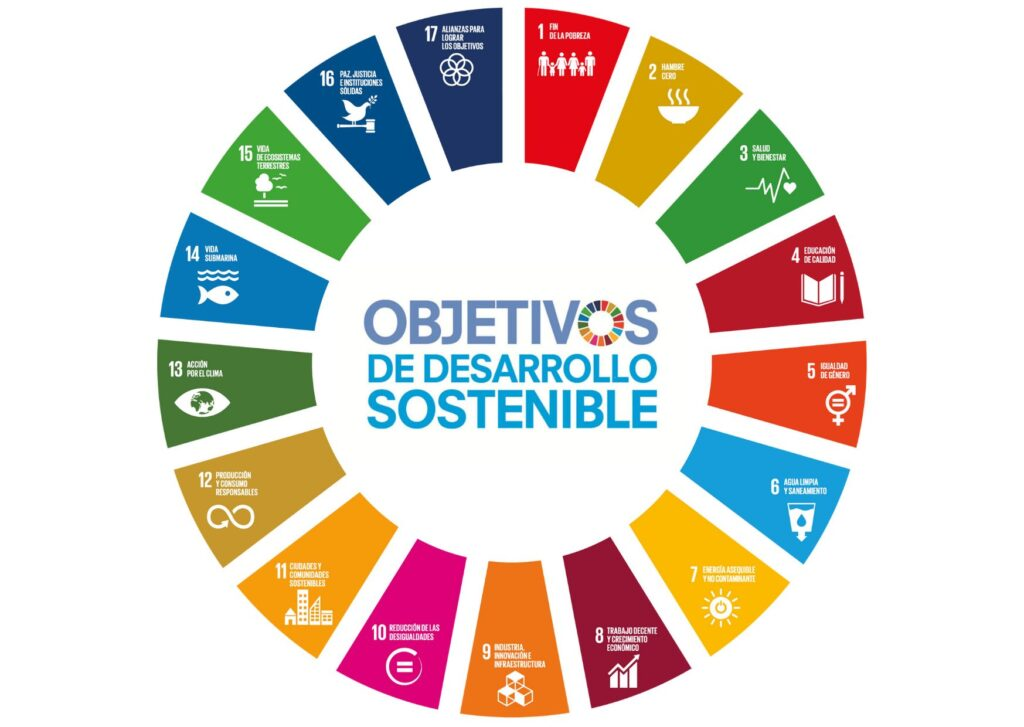
\includegraphics[width=0.7\linewidth]{img/ODS.jpg}
    \caption{Objetivos ODS del Desarrollo Sostenible}
    \label{fig:ODS}
\end{figure}





\bibliographystyle{apalike}
\bibliography{bibliografiaAnexos}

\end{document}
